% !TEX encoding = UTF-8
% !TEX TS-program = pdflatex
% !TEX root = ../Tesi.tex
% !TEX spellcheck = it-IT

%************************************************

%************************************************
In questo capitolo si descriverà la progettazione e l’esecuzione della sperimentazione. 

Obiettivo di questo capitolo è quello di valutare l’efficacia dell'approccio realizzato al fine di comprendere se e come i dati strutturati, di cui un sito web si compone,  possano essere combinati con dati non strutturati, come quelli testuali, al fine di migliorare il processo di clustering e valutare in dettaglio le cause di un eventuale successo o insuccesso delle tecniche utilizzate.
A tal fine si confornteranno le performance degli algoritmi di clustering basati su rappresentazione a grafo con algoritmi di clustering basati su rappresentazione vettoriale contenente informazioni sulla struttura del grafo stesso.
 
Questa tesi rappresenta un lavoro preliminare utile a comprendere la bontà della soluzione proposta e quindi decidere se proseguire gli studi in questa direzione o definire strategie alternative.

Si descrivono di seguito i dataset e le configurazioni degli algoritmi di clustering su cui sono realizzate le sperimentazioni e le metriche utilizzate per valutare la qualità dei cluster estratti. Infine verranno mostrati una serie di grafici e tabelle utili a comparare i risultati ottenuti al variare delle configurazioni.

%A tal fine si è deciso di valutare la qualità dell'approccio proposto confrontando le prestazioni di alcuni algoritmi di clustering basati su due differenti tipi di rappresentazione: rappresentazione a grafo e rappresentazione vettoriale.
\section{Dataset}
La sperimentazione è stata effettuata sfruttando i dati provenienti da siti web appartenenti a tre importanti dipartimenti di Computer Science:
%i risultati ottenuti attraverso l'applicazione di diversi algoritmi di clustering su dataset ottenuti da differenti rappresentazioni. L'algoritmo è stato testato effettuando il crawling di $3$ siti web, che sono stati poi etichettati manualmente per ricavare le metriche necessarie alla valutazione della tesi proposta.

\begin{itemize}

\item Dipartimento di Computer Science dell'università di Urbana, IL:\\
\texttt{www.cs.illinois.edu}\\
Il crawling è stato lanciato con profondità massima $10$, e immagazzinando un massimo di $10.000$ termini per ogni pagina esplorata. Il grafo web estratto si compone di $728$ pagine web e $16993$ hyperlink. Dal grafo sono state poi generate $10.000$ sequenze di lunghezza massima $10$.

\item Dipartimento di Computer Science dell'università di Stanford, CA: \texttt{cs.stanford.edu} \\Il crawling è stato effettuato con profondità massima $10$, e immagazzinando un massimo di $10.000$ termini per ogni pagina esplorata. Il grafo web estratto si compone di $1458$ pagine web e $99686$ hyperlink. Dal grafo sono state poi generate $10.000$ sequenze di lunghezza massima $10$.

\item Dipartimento di Computer Science del  Massachusetts Institute of Technology a Cambridge, MA: \texttt{eecs.mit.edu} \\ Il crawling è stato lanciato con profondità massima $10$, e immagazzinando un massimo di $10.000$ termini per ogni pagina esplorata. Il grafo web estratto si compone di $1745$ pagine web e $63937$ hyperlink. Dal grafo sono state poi generate $10.000$ sequenze di lunghezza massima $10$.

\item Dipartimento di Computer Science dell'università di Princeton, NJ: \texttt{cs.princeton.edu} \\ Il crawling è stato lanciato con profondità massima $7$, e immagazzinando un massimo di $10.000$ termini per ogni pagina esplorata. Il grafo web estratto si compone di $16378$ pagine web e $206985$ hyperlink. Dal grafo sono state poi generate $10.000$ sequenze di lunghezza massima $10$.

\item Dipartimento di Computer Science dell'università di Oxford, UK:\\ \texttt{cs.ox.ac.uk} \\ Il crawling è stato lanciato con profondità massima $5$, e immagazzinando un massimo di $10.000$ termini per ogni pagina esplorata. Il grafo web estratto si compone di $4183$ pagine web e $27954$ hyperlink. Dal grafo sono state poi generate $10.000$ sequenze di lunghezza massima $10$.

\end{itemize}

La scelta dei precedenti siti è dovuta a ragioni di confidenza con il dominio applicativo. Infatti la valutazione dei risultati sperimentali ha richiesto, oltre che il crawling dei siti web sopracitati anche una fase di etichettatura delle pagine web al fine di generare una ground truth.

Inoltre per ogni sito web sono stati estratti due differenti grafi web:
\begin{itemize}
\item \textbf{Web graph no-constraint (nc)}. Il grafo web $G_{nc}=(V,E)$ rappresenta fedelmente il sito web. In particolare $V$ rappresenta l'insieme delle pagine web appartenenti al sito ed $E$ è l'insieme di tutte le coppie $(i,j)$ per i quali la pagina con url $i$ contiene un outlink alla pagina con url $j$.
\item \textbf{Web graph list-constraint (lc)}. Il grafo web $G_{ls}=(V,E)$ è filtrato eliminando tutti quegli archi $(i,j) \in E$ per i quali l'url $j$ non è contenuto in nessuna lista web nella pagina con url $i$ (vedi Sezione \color{red} metti sezione \color{black}).
\end{itemize}

%Si descrivono di seguito le metriche utilizzate per valutare la qualità dei cluster estratti, la scelta delle modalità di esecuzione più interessanti e si mostreranno una serie di tabelle e grafici contenenti i risultati ottenuti. 


\section{Metriche}
Valutare le performance di un algoritmo di clustering non è semplice come contare il numero di errori o calcolare metriche quali $Precision$ e $Recall$ di un algoritmo di apprendimento supervisionato. In particolare, le metriche di valutazione non dovrebbero prendere in considerazione gli specifici valori delle label. Queste dovrebbero piuttosto considerare se il raggruppamento generato dall'algortimo definisce una separazione dei dati similmente a quanto fornito nella \textit{ground truth}, ovvero il vero valore delle label, o soddisfare qualche assunzione, come ad esempio che membri dello stesso cluster siano più simili rispetto a quelli di cluster differenti, utilizzando una data funzione di similarità. Di seguito si elencano le metriche utilizzate per valutare la qualità dei cluster prodotti.

\begin{itemize}
\item \textbf{Omogeneità}: nota la ground truth (ossia l'insieme dei cluster ideali), questo valore rappresenta quanto ogni cluster appreso sia omogeneo,
ossia quanto gli elementi dello stesso cluster appartengono alla setssa classe.
Formalmente l'omogeneità può essere definita come segue:
\begin{equation}
h = 1 - \frac{H(C|K)}{H(C)};
\end{equation}
dove $H(C|K)$ è l'entropia condizionata delle classi date le assegnazioni dei cluster e $H(C)$ è l'entropia delle classi, ossia:
\begin{equation}
H(C|K) = - \sum\limits_{c=1}^{|C|} \sum\limits_{k=1}^{|K|} \frac{n_{c,k}{n}} \cdot \log \left( \frac{n_{c,k}}{n_k}\right)
\end{equation}
\label{hck}

\begin{equation}
H(C) = \sum\limits_{c=1}^{|C|} \frac{n_c}{n} \cdot \log \left( \frac{n_{c}}{n}\right)
\end{equation}
\label{hc}
con $n$ il numero totale delle pagine, e $n_c$ ed $n_k$ il numero delle pagine appartenenti alla classe $c$ o al cluster $k$, ed infine $n_{c,k}$ sono le pagine della classe $c$ assegnate al cluster $k$. In una situazione ideale l'omogeneità assume valore 1.  \cite{Rosenberg07}
\item \textbf{Completezza}: è una misura simmetrica all'Omogeneità. In modo da soddisfare i criteri di completezza un algoritmo di clustering deve assegnare tutti gli elementi di una data classe ad un unico cluster. Per valutare la completezza è necessario esaminare la distribuzione degli assegnamenti di ogni classe. In particolare in una soluzione perfetta ogni distribuzione di classe dovrebbe convergere in un cluster.
%nota la ground truth, indica se tutti i membri di una classe sono stati assegnati allo stesso cluster. Da notare che se ad esempio tutte le pagine fossero assegnate ad un unico grande cluster, la \textit{Completezza} sarebbe massima.
Formalmente la \textit{Completezza} può essere così formulata:
\begin{equation}
c = 1 - \frac{H(C|K)}{H(K)}
\end{equation}
dove $H(C|K)$ è definita nell'equazione \ref{hck} e $H(K)$ è l'entropia dei cluster. Come nel caso dell'Omogeneità la Completezza di una soluzione ideale assume valore 1.
\item \textbf{V-Measure}: è una misura basata sull'entropia che esplicitamente calcola quanto i criteri di omogeneità e completezza sono stati soddifatti. Essa è computata come la media armonica fra Omogeneità e Completezza, così come Precisione e Richiamo sono combinati nel calcolo del F-Measure:
\begin{equation}
v = 2 \cdot \frac{h \cdot c}{h + c}
\end{equation}

\item \textbf{Adjusted Rand Index (ARI)}: nota la ground truth e gli assegnamenti restituiti da un algoritmo di clustering, l'ARI calcola la similarità tra i due insiemi ignorando le permutazioni \cite{Santos09}. 

Da un punto di vista matematico l'ARI misura l'accuratezza del clustering, ossia la percentuale di coppie di oggetti per i quali due algoritmi di clustering concordano sull'assegnazione. 
In particolare, dato $C$ l'insieme degli assegmaneti ideali (ground truth) e $K$ l'insieme delle label predette, allora è possibile calcolare il \textbf{Random Index}:
%Il \textbf{Random Index} è dato da:
\begin{equation}
RI = \frac{a + b}{C_2^n}
\end{equation}
Dove:
\\
- $a$ è il numero di coppie di elementi che si trovano sia in $c$ che in $K$
\\
- $b$ è il numero di coppie di elementi che si trovano in insiemi diversi in $C$ e in insiemi diversi in $K$.
\\
- $C_2^n$ è il numero totale di tutte le possibili coppie nel dataset. 
\\
%Il $RI$ non garantisce che le assegnazioni casuali abbiano valori prossimi allo $0$.

Un problema del $RI$ è che cluster cumputati in modo casuale non assumono un indice costante (per esempio 0).
\\ A tal fine è definito l'Adjusted Random Index:
\begin{equation}
ARI = \frac{RI - E[RI]}{\max (RI) - E[RI]}
\end{equation}
Questa misura garantisce che cluster generati in modo casuale abbiano un valore ARI prossimi allo 0.
Differentemente dalle precedenti misure l'ARI assume valori tra $-1$ e $1$. %Risultati prossimi allo $0$ rappresentano una assegnazione casuale delle etichette.

\item \textbf{Mutual Information (MI)}: nota la ground truth e le asseganzioni dell'algoritmo di clustering, la \textit{Mutual Information} è una funzione che misura la corrispondenza delle due informazioni, ignorando le permutazioni. 
\\
Anche qui, una assegnazione uniforme (o casuale) dei cluster avrà valori prossimi allo $0$, evidenziando l'indipendenza delle due informazioni, mentre valori prossimi a $1$ indicano una corrispondenza significativa.
\\
Dati due assegnamenti di pari lunghezza, $U$ e $V$, la loro entropia è la quantità di incertezza per una partizione, definita da:
\begin{equation}
H(U) = \sum\limits_{i=1}^{|U|} P(i)\log (P(i))
\end{equation}
Dove $P(i) = \frac{|U_i|}{N}$ è la probabilità che un oggetto preso a caso da $U$ appartenga alla classe $U_i$. Similmente per $V$:
\begin{equation}
H(V) = \sum\limits_{j=1}^{|V|} P'(j)\log (P'(j))
\end{equation}
Con $P'(j) = \frac{|V_j|}{N}$. La Mutual Information p definita come:
\begin{equation}
MI(U,V) = \sum\limits_{i=1}^{|U|}\sum\limits_{j=1}^{|V|} P(i,j)\log \left( \frac{P(i,j)}{P(i)P'(j)} \right)
\end{equation}

\end{itemize}

Per le metriche riportate è degno di nota che nessuna assunzione viene fatta sulla struttura dei cluster, quindi possono essere utilizzate con algoritmi che identificano cluster di forma diversa.
\\
Queste, ad eccezione dell'ARI, essendo misure probabilistiche i valori possibili spaziano nell'intervallo $(0,1)$. 
%Nelle metriche presentate, fatta eccezione per l'Adjusted Rand Index, $0.0$ rappresenta il valore peggiore, mentre $1.0$ il perfect score. Questi valori offrono una interpretazione intuitiva e può aiutare alla scoperta degli errori commessi nella assegnazione. Fra i vantaggi è degno di nota che nessuna assunzione viene fatta sulla struttura dei cluster, quindi possono essere utilizzate con algoritmi che identificano cluster di forma diversa.


\paragraph{Silhouette}: misura la forza di ogni cluster~\cite{Rousseeuw87}. Essa può essere usata per calcolare la qualità dei cluster anche quando la Ground Truth non è nota.
Formalmente la Silhouette può essere così definita:
\begin{equation}
s = \frac{b - a}{\max (a,b)}
\end{equation}
dove:
\\
- $a$ = la distanza media tra un vettore e tutti gli altri nella stessa classe
\\
- $b$ = la distanza media tra un vettore e tutti gli altri nella classe più vicina

La Silhouette può variare da $-1$, per cluster non definiti, a $1$ per cluster densamente connessi. Un valore intorno allo $0$ indica cluster sovrapposti. In generale cluster convessi o molto densi come quelli ottenuti con DBSCAN, assumono alti valori.
%Tende comunque ad essere maggiore per cluster convessi, o con alta densità, come quelli ottenuti con DBSCAN.
\section{Configurazioni}
Si descrivono di seguito le configurazioni utilizzate per gli algoritmi di clustering utilizzati durante la fase di sperimentazione. 

\subsection{Community Detection}
Per gli algoritmi di clustering basati su grafo sono stati utilizzati \textit{Walk Trap} e \textit{Fastgreedy}. Questi rappresentano gli algoritmi più comunemente utilizzati in applicazioni come \textit{Social Network Mining} per estrarre Web Community.

Fastgreedy non richiede parametri specifici, tuttavia per ogni sito web è stata definita un'altezza entro cui tagliare il dendogramma in modo tale che il numero dei cluster restituiti sia simile al numero dei cluster della groud truth. WalkTrap invece richiede in input la lunghezza dei Random Walk.



La tabella \ref{tabwebsites} mostra per ogni sito web oggetto di analisi i parametri utilizzati.

\begin{table}[]
\centering
\caption{My caption}
\label{tabwebsites}
\begin{tabular}{|l|l|l|l|l|l|}
\hline
 \textbf{Web site}& \textbf{ran walk len} & \textbf{dendr.cut} & \textbf{num. real clusters}\\ \hline
\texttt{cs.illinois.edu}  & 3 &   15 & 16 \\ \hline
\texttt{cs.stanford.edu}& 3 & 10 & 13 \\ \hline
\texttt{eecs.mit.edu} & 3 & 15 & 16 \\ \hline
\texttt{cs.princeton} & 4 & 20 & 29 \\ \hline
\texttt{cs.ox.ac.uk} & 4 & 20 & 26 \\ \hline
\end{tabular}
\end{table}

\subsection{URL Embedding}
Considerando i Random Walk generati sul grafo come frasi, è possibile applicare algoritmi di Word Embedding per raggruppare le pagine sulla base del contesto in cui appaiono, ovvero le pagine che più verosimilmente appariranno insieme nelle sequenze.
\\
Le sequenze di Random Walk sono state usate per apprendere rappresentazioni vettoriali delle pagine Web. La fase di URL embedding è stata effetuata utilizzando l'algoritmo Word2vec, \cite{gensim} (esaminato in Sezione \ref{word2vec}) modificando alcuni parametri e lasciando invariato altri.
\\

I parametri personalizzati sono:
\begin{itemize}
\item \textbf{min-count}: tutte le parole (o URL) con frequenza di occorrenza minore i questo valore vengono ignorate.
\item \textbf{window} rappresenta la distanza massima tra l'URL corrente e quello predetto all'interno di una frase.
\item \textbf{negative} Nella fase di embedding di una URL, viene calcolato il rapporto tra la similarità del contesto con la parola e la sommatoria di tutte le similarità tra la parola e gli altri contesti. Più precisamente:
\begin{equation}
\frac{v_c \cdot v_w}{\sum\limits_{c \in C} v_c \cdot v_w}
\end{equation}
Questa operazione può essere molto lenta. Per accelerare il processo possono venir scelti $n$ contesti casuali da confrontare. Questo parametro, se maggiore di $0$, rappresenta il numero di vettori da confrontare.
\item \textbf{sg} definisce l'algoritmo di apprendimento, di default viene usato \textit{CBOW}, mentre se impostato a $1$ utilizza \textit{skip-gram} \cite{Mikolov13}. Per lo scopo della sperimentazione si imposterà questo valore a  CBOW.
\end{itemize}

Sulle rappresentazioni vettoriali estratte sono stati applicati gli algoritmi HDBSCAN e K-MEANS.
Di seguito si definiscono i parametri utilizzati per ogni sito web: 
\begin{itemize}
\begin{figure}[h!]
	\centering
	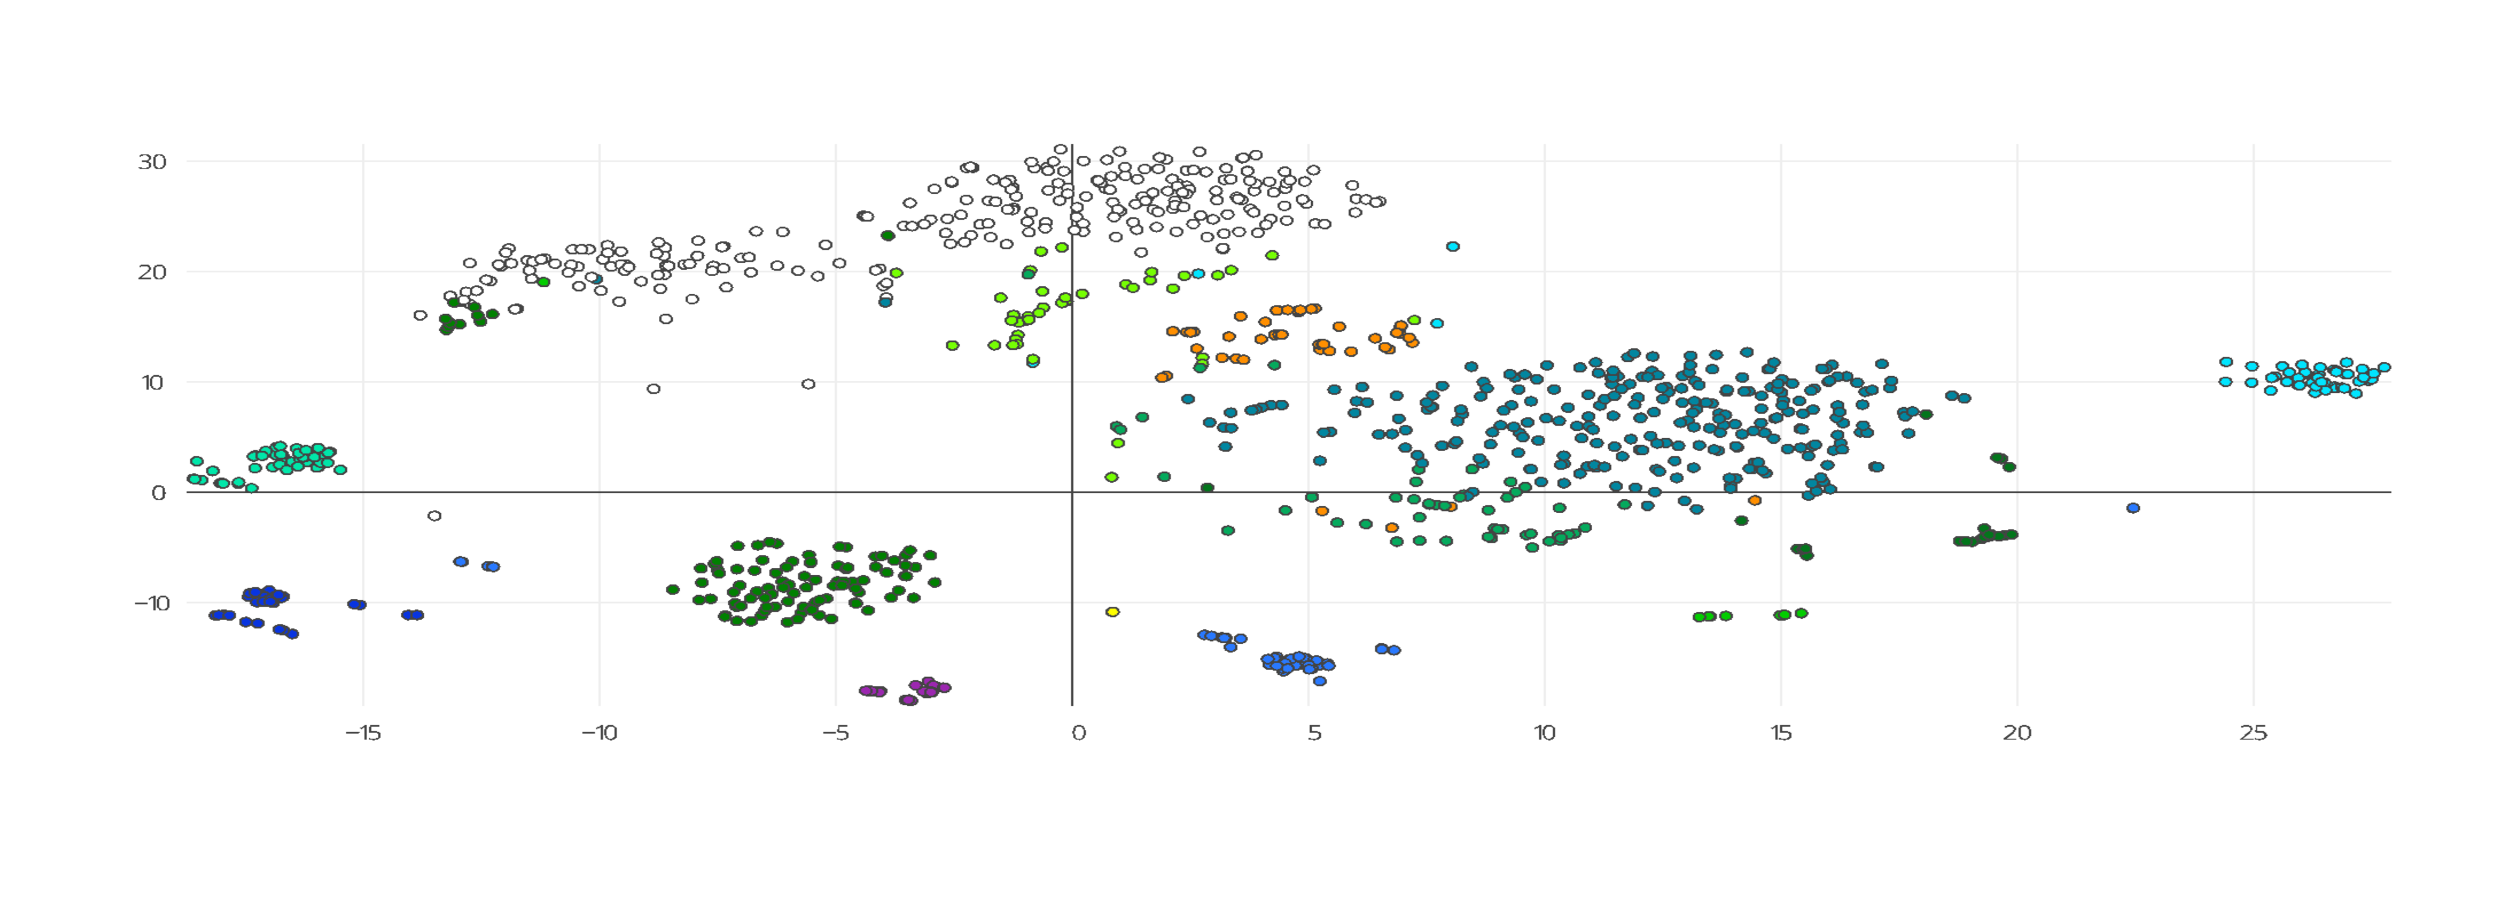
\includegraphics[width = 130mm, height=93mm]{lc_embedding_km.png}
	\caption{Rappresentazione del sito \texttt{cs.illinois.edu}, clusterizzato con K-Means.}
	\label{nc_embedding_km}
\end{figure}

\item \texttt{cs.illinois.edu} è stata impostato un \textit{min-count} pari a $1$, \textit{window} con valore $5$ ed è stato utilizzato \textit{skip-gram} con $5$ \textit{negative} sampling. Gli algoritmi testati sono stati: DBSCAN con $\epsilon = 0.9$ ed \textit{min-samples}$ = 4$; HDBSCAN con \textit{min-cluster-size}$=6$; K-Means con numero di cluster pari a $15$. 
\item \texttt{cs.stanford.edu} è stata impostato un \textit{min-count} pari a $1$, \textit{window} con valore $5$ ed è stato utilizzato \textit{skip-gram} con $5$ \textit{negative} sampling. Gli algoritmi testati sono stati: DBSCAN con $\epsilon = 0.9$ ed \textit{min-samples}$ = 7$; HDBSCAN con \textit{min-cluster-size}$=10$; K-Means con numero di cluster pari a $10$. Per il dataset delle liste: DBSCAN con $\epsilon = 1.6$ ed \textit{min-samples}$ = 3$; HDBSCAN con \textit{min-cluster-size}$=5$; K-Means con numero di cluster pari a $10$.
\item \texttt{eecs.mit.edu} è stata impostato un \textit{min-count} pari a $1$, \textit{window} con valore $5$ ed è stato utilizzato \textit{skip-gram} con $5$ \textit{negative} sampling. Gli algoritmi testati sono stati: DBSCAN con $\epsilon = 1.0$ ed \textit{min-samples}$ = 10$; HDBSCAN con \textit{min-cluster-size}$=10$; K-Means con numero di cluster pari a $15$. Per il dataset delle liste: DBSCAN con $\epsilon = 1.5$ ed \textit{min-samples}$ = 5$; HDBSCAN con \textit{min-cluster-size}$=13$; K-Means con numero di cluster pari a $15$.
\item \texttt{cs.princeton.edu} è stata impostato un \textit{min-count} pari a $1$, \textit{window} con valore $5$ ed è stato utilizzato \textit{skip-gram} con $5$ \textit{negative} sampling. Gli algoritmi testati sono stati: DBSCAN con $\epsilon = 0.8$ ed \textit{min-samples}$ = 7$; HDBSCAN con \textit{min-cluster-size}$=10$; K-Means con numero di cluster pari a $30$. Per il dataset delle liste: DBSCAN con $\epsilon = 0.7$ ed \textit{min-samples}$ = 5$; HDBSCAN con \textit{min-cluster-size}$=8$; K-Means con numero di cluster pari a $25$.
\item \texttt{cs.ox.ac.uk} è stata impostato un \textit{min-count} pari a $1$, \textit{window} con valore $5$ ed è stato utilizzato \textit{skip-gram} con $5$ \textit{negative} sampling. Gli algoritmi testati sono stati: DBSCAN con $\epsilon = 0.8$ ed \textit{min-samples}$ = 7$; HDBSCAN con \textit{min-cluster-size}$=10$; K-Means con numero di cluster pari a $30$. Per il dataset delle liste: DBSCAN con $\epsilon = 0.7$ ed \textit{min-samples}$ = 5$; HDBSCAN con \textit{min-cluster-size}$=8$; K-Means con numero di cluster pari a $25$.
\end{itemize}

\subsection{Text Mining}
Sono state utilizzate tecniche di Text Mining per il clustering basato sul contenuto testuale. I contenuti all'interno di uno stesso sito web avranno una struttura e termini comuni, differenziandosi al variare dell'argomento trattato. La struttura gerarchica di un sito web organizza solitamente le pagine in sezioni simili. Questa metodologia tuttavia, considera solo l'informazione testuale, assumendo che i termini all'interno del sito web siano indipendenti l'uno dall'altro così come i documenti, ignorando le relazioni interdipendenti tra questi. Il web si discosta dall'analisi classica dei documenti proprio per le relazioni che intercorrono tra le pagine, tuttavia l'analisi testuale rimane molto importante.
\\
Nella fase di sperimentazione è stata utilizzata una rappresentazione vettoriale della frequenza dei termini all'interno dell'insieme delle pagine web, calcolata con la tecnica della \textit{frequency–inverse document frequency} (tf-idf).

I parametri personalizzati per la costruzione dell matrice documenti-termini con funzione di peso \textit{idf} sono stati:
\begin{itemize}
\item \textbf{max-df}: questo valore rappresenta la massima frequenza, all'interno dei documenti, che un termine può avere per essere utilizzato nella matrice tf-idf. Se un termine appare molte volte nel corpus, molto probabilmente avrà poco significato.
\item \textbf{min-df}: indica il numero minimo di documenti in cui un termine dovrà apparire per essere considerato.
\item \textbf{ngram-range}: vengono presi in considerazioni gli n-grammi di lunghezza compresa nell'intervallo specificato in questo parametro. Un n-gramma è una sottosequenza  di $n$ elementi di un'altra.
\end{itemize}

I cluster estratti sono stati ottenuti nel seguente modo:
\begin{itemize}
\item \texttt{cs.illinois.edu}
Sul dataset del sito, costituito da $728$ pagine e $433$ termini, il corpus è stato ripulito delle stopword, stemmatizzato ed è stato impostato il \textit{max-df} all'80\%, il \textit{min-df} a $0.1$ e sono stati considerati solo uni-grammi, bi-grammi e tri-grammi. Se i termini appaiono in più dell'80\% dei documenti, probabilmente avrà poco significato, lo stesso se appare troppe poche volte. Gli algoritmi testati sono stati: DBSCAN con $\epsilon = 0.9$ ed \textit{min-samples}$ = 4$; HDBSCAN con \textit{min-cluster-size}$=4$; K-Means con numero di cluster pari a $15$. \\Sul Dataset costruito estraendo le liste: DBSCAN con $\epsilon = 0.7$ ed \textit{min-samples}$ = 4$; HDBSCAN con \textit{min-cluster-size}$=7$; K-Means con numero di cluster pari a $15$. 
\item \texttt{cs.stanford.edu}
Sul dataset del sito, costituito da $1458$ pagine e $843$ termini, il corpus è stato ripulito delle stopword, stemmatizzato ed è stato impostato il \textit{max-df} all'80\%, il \textit{min-df} a $0.1$ e sono stati considerati solo uni-grammi, bi-grammi e tri-grammi. Se i termini appaiono in più dell'80\% dei documenti, probabilmente avrà poco significato, lo stesso se appare troppe poche volte. Gli algoritmi testati sono stati: DBSCAN con $\epsilon = 0.3$ ed \textit{min-samples}$ = 5$; HDBSCAN con \textit{min-cluster-size}$=15$; K-Means con numero di cluster pari a $10$. \\Sul Dataset costruito estraendo le liste: DBSCAN con $\epsilon = 0.5$ ed \textit{min-samples}$ = 3$; HDBSCAN con \textit{min-cluster-size}$=5$; K-Means con numero di cluster pari a $10$. 
\item \texttt{eecs.mit.edu}
Sul dataset del sito, costituito da $1745$ pagine e $354$ termini, il corpus è stato ripulito delle stopword, stemmatizzato ed è stato impostato il \textit{max-df} all'80\%, il \textit{min-df} a $0.1$ e sono stati considerati solo uni-grammi, bi-grammi e tri-grammi. Se i termini appaiono in più dell'80\% dei documenti, probabilmente avrà poco significato, lo stesso se appare troppe poche volte. Gli algoritmi testati sono stati: DBSCAN con $\epsilon = 0.9$ ed \textit{min-samples}$ = 9$; HDBSCAN con \textit{min-cluster-size}$=15$; K-Means con numero di cluster pari a $15$. \\Sul Dataset costruito estraendo le liste: DBSCAN con $\epsilon = 0.9$ ed \textit{min-samples}$ = 6$; HDBSCAN con \textit{min-cluster-size}$=9$; K-Means con numero di cluster pari a $15$. 
\item \texttt{cs.princeton.edu}
Sul dataset del sito, costituito da $16378$ pagine e $470$ termini, il corpus è stato ripulito delle stopword, stemmatizzato ed è stato impostato il \textit{max-df} all'80\%, il \textit{min-df} a $0.1$ e sono stati considerati solo uni-grammi, bi-grammi e tri-grammi. Se i termini appaiono in più dell'80\% dei documenti, probabilmente avrà poco significato, lo stesso se appare troppe poche volte. Gli algoritmi testati sono stati: DBSCAN con $\epsilon = 0.3$ ed \textit{min-samples}$ = 5$; HDBSCAN con \textit{min-cluster-size}$=15$; K-Means con numero di cluster pari a $20$. \\Sul Dataset costruito estraendo le liste: DBSCAN con $\epsilon = 0.9$ ed \textit{min-samples}$ = 6$; HDBSCAN con \textit{min-cluster-size}$=15$; K-Means con numero di cluster pari a $20$.  
\item \texttt{cs.ox.ac.uk}
Sul dataset del sito, costituito da $3951$ pagine e $363$ termini, il corpus è stato ripulito delle stopword, stemmatizzato ed è stato impostato il \textit{max-df} all'80\%, il \textit{min-df} a $0.1$ e sono stati considerati solo uni-grammi, bi-grammi e tri-grammi. Se i termini appaiono in più dell'80\% dei documenti, probabilmente avrà poco significato, lo stesso se appare troppe poche volte. Gli algoritmi testati sono stati: DBSCAN con $\epsilon = 0.3$ ed \textit{min-samples}$ = 5$; HDBSCAN con \textit{min-cluster-size}$=15$; K-Means con numero di cluster pari a $20$. \\Sul Dataset costruito estraendo le liste: DBSCAN con $\epsilon = 0.7$ ed \textit{min-samples}$ = 7$; HDBSCAN con \textit{min-cluster-size}$=7$; K-Means con numero di cluster pari a $20$. 
\end{itemize}

\subsection{Embedding e Text Mining}
La terza ed ultima configurazione analizzata è rappresentata dalla combinazione nella rappresentazione vettoriale di informazioni riguardanti il contenuto testuale delle pagine web e la struttura del sito web. Questo è realizzato attraverso la combinazione di rappresentazioni vettoriali ottenute con algoritmi di Word Embedding e rappresentazioni vettoriali ottenute con algoritmi derivanti dall'analisi del contenuto testuale. 

Di seguito si definiscono i parametri e gli algoritmi utilizzati in questa configurazione:
\begin{itemize}
\item \texttt{cs.illinois.edu} I vettori di word2vec sono stati generati di dimensione $48$, mentre i vettori-riga documenti sono stati ridotti con \textit{TruncateSVD} a dimensione $50$. Gli algoritmi testati sono stati: HDBSCAN con \textit{min-cluster-size}$=7$; K-Means con numero di cluster pari a $15$.
\item \texttt{cs.stanford.edu} I vettori di word2vec sono stati generati di dimensione $48$, mentre i vettori-riga documenti sono stati ridotti con \textit{TruncateSVD} a dimensione $50$. Gli algoritmi testati sono stati: HDBSCAN con \textit{min-cluster-size}$=10$; K-Means con numero di cluster pari a $15$. 
\item \texttt{eecs.mit.edu} I vettori di word2vec sono stati generati di dimensione $48$, mentre i vettori-riga documenti sono stati ridotti con \textit{TruncateSVD} a dimensione $50$. Gli algoritmi testati sono stati: HDBSCAN con \textit{min-cluster-size}$=14$; K-Means con numero di cluster pari a $15$. 
\item \texttt{cs.princeton.edu} I vettori di word2vec sono stati generati di dimensione $48$, mentre i vettori-riga documenti sono stati ridotti con \textit{TruncateSVD} a dimensione $50$. Gli algoritmi testati sono stati: HDBSCAN con \textit{min-cluster-size}$=14$; K-Means con numero di cluster pari a $20$. 
\item \texttt{cs.ox.ac.uk} I vettori di Word2vec sono stati generati di dimensione $48$, mentre i vettori-riga documenti sono stati ridotti con \textit{TruncateSVD} a dimensione $50$. Gli algoritmi testati sono stati: HDBSCAN con \textit{min-cluster-size}$=14$; K-Means con numero di cluster pari a $20$.
\end{itemize}

\section{Analisi dei risultati}
Di seguito si confrontano i risultati degli algoritmi di clustering basati su grafo con quelli basati su rappresentazioni vettoriali al variare del grafo web (list-constraint vs no-constraint).
Inoltre per gli algoritmi di clustering basati su vettori si analizzano le prestazioni degli algoritmi al variare delle rappresentazioni vettoriali (Url-embedding, Tf-idf, Url-embeddig + tf-idf).

La divisione del grafo in Community può essere effettuata seguendo diversi approcci, tuttavia la rete costruita su un sito web è caratterizzata solitamente da un numero elevato di collegamenti tra pagine, il quale suggerisce l'utilizzo di alcune tipologie piuttosto che altre. Infatti misure come la betweenness non hanno restituito risultati significativi.
Dalla scelta di apprendere le rappresentazioni vettoriali delle relazioni invece di utilizzare algoritmi di Community Detection del grafo, sono derivati dei vantaggi. Innanzitutto gli algoritmi di partizionamento dei grafi hanno complessità NP-completa, ovvero necessitano di un tempo esponenziale nella dimensione dell'input. Nel contesto del Web Mining la dimensione del dataset può crescere enormemente ed avere soluzioni più efficienti costituisce senz'altro una priorità. 
\\
In tutti i casi di seguito riportati sono stati generati grafi sia in modalità classica, che attraverso l'estrazione delle liste. Nel primo caso i dataset saranno chiamati \textbf{''nc''} (no-costraint, senza vincoli), mentre nel secondo caso \textbf{''lc''} (list-costraint, con il vincolo delle liste (vedere sezione \ref{liste}). Dove omessa, la configurazione è rimasta invariata.

\subsection{cs.illinois.edu}
\begin{table}[H]
	\begin{tabular}{| l | c | c | c | c | c | c |}
	\hline
	\textbf{Illinois}  & \textbf{Hom} & \textbf{Com} & \textbf{V-M}  & \textbf{ARI}  & \textbf{MI} & \textbf{Silh}\\ [2ex] \hline
	\textbf{G-nc WT} & 0.6471 & 0.6585 & 0.6527 & 0.4363 & 0.6281 & //\\ [2ex]
	 \hline
	\textbf{G-nc FG} & 0.5518 & \textbf{0.8563} & 0.6711 & 0.5764 & 0.5354 & //\\ [2ex]
	 \hline	
	\textbf{G-lc WT} & 0.5093 & 0.4892 & 0.4991 & 0.2762 & 0.4722 & //\\ [2ex]
	 \hline	
	\textbf{G-lc FG} & 0.5522 & 0.6035 & 0.5767 & 0.3656 & 0.5382 & //\\ [2ex]
	\hline
	
	\textbf{E-nc dbscan} & 0.5553 & 0.6579 & 0.6023 & 0.4487 & 0.5234 & 0.2588\\ [2ex]
	 \hline 
	\textbf{E-nc hdbscan} & 0.5759 & 0.6720 & 0.6203 & 0.5282 & 0.5525 & 0.2573\\ [2ex]
	 \hline
	\textbf{E-nc Kmeans} & 0.8238 & 0.7575 & 0.7892 & 0.7883 & 0.7423 & 0.3131\\ [2ex]
	 \hline	
	\textbf{E-lc dbscan} & 0.4163 & 0.5922 & 0.4889 & 0.2250 & 0.3935 & 0.1320\\ [2ex]
	\hline
	\textbf{E-lc hdbscan} & 0.4760 & 0.5067 & 0.4908 & 0.2275 & 0.4515 & 0.1054\\ [2ex]
	\hline
	\textbf{E-lc Kmeans} & 0.8095 & 0.6593 & 0.7267 & 0.6189 & 0.6473 & 0.2281\\ [2ex]
	\hline
	
	\textbf{T dbscan} & 0.5601 & 0.5962 & 0.5776 & 0.4078 & 0.5346 & 0.1242\\ [2ex]
	 \hline 
	\textbf{T hdbscan} & 0.5152 & 0.6029 & 0.5556 & 0.3862 & 0.4858 & 0.0881\\ [2ex]
	 \hline
	\textbf{T Kmeans} & 0.7619 & 0.5814 & 0.6596 & 0.3184 & 0.5586 & 0.1767\\ [2ex]
	 \hline		
	\textbf{ET-nc hdbscan} & 0.7327 & 0.7534 & 0.7429 & 0.7204 & 0.7186 & 0.2070\\ [2ex]
	 \hline 
	\textbf{ET-nc Kmeans} & \textbf{0.8812} & 0.8069 & \textbf{0.8424} & \textbf{0.8299} & \textbf{0.7949} & \textbf{0.3198}\\ [2ex]
	 \hline
	\textbf{ET-lc hdbscan} & 0.6541 & 0.6129 & 0.6328 & 0.3249 & 0.5992 & 0.1203\\ [2ex]
	\hline
	\textbf{ET-lc Kmeans} & 0.8548 & 0.6885 & 0.7627 & 0.6488 & 0.6773 & 0.2573\\ [2ex]
	\hline	
	
	\end{tabular}
	\caption{Risultati sperimentazione del sito \texttt{cs.illinois.edu}}
	\label{metricheIll}
\end{table}

\begin{figure}[ht!]
	\centering
	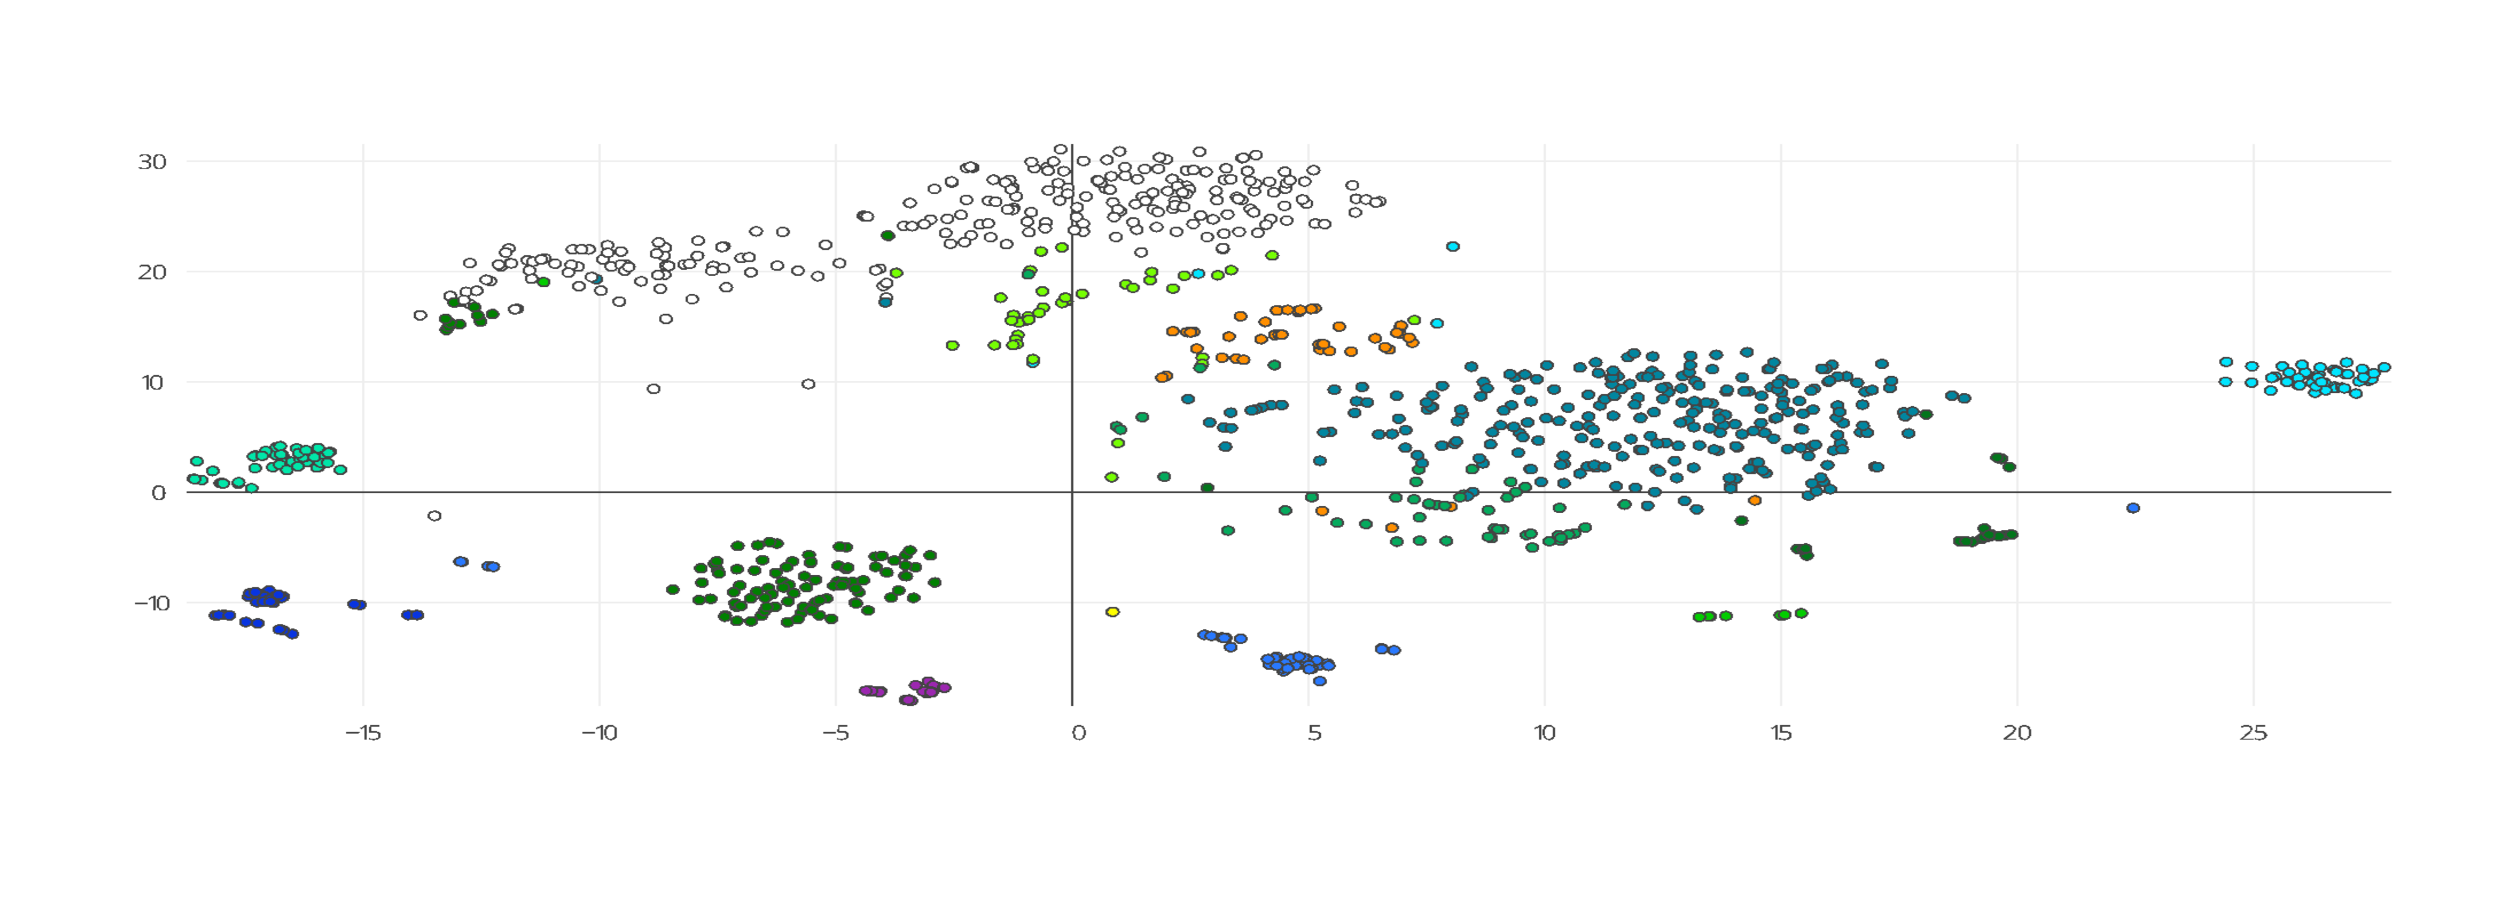
\includegraphics[width = 130mm, height=75mm]{lc_embedding_km.png}
	\caption{Rappresentazione del sito \texttt{cs.illinois.edu}, clusterizzato con K-Means.}
	\label{nc_embedding_km}
\end{figure}

I risultati hanno evidenziato che l'analisi singola, sia della correlazione tra le pagine sia del contenuto testuale, può non bastare a codificare esaustivamente la conoscenza che una pagina web può offrire. Entrambe le informazioni sono rilevanti ed andrebbero processate insieme in quanto le informazioni codificate nelle due tipologie di vettori sono complementari.
\color{red}Le sperimentazioni effettuate sul grafo intero (\textbf{nc}) e sul grafo costruito unicamente con gli hyperlink nelle liste (\textbf{lc}), hanno restituito risultati migliori delle altre configurazioni. \color{black}

Dai risultati si osserva come gli algoritmi di clustering basati su rappresentazione vettoriale ottengono per il sito cs.iillinois.edu migliori performace degli algoritmi di clustering basati su rappresentazione a grafo. SCRIVERE EVENTUALMENTE PERCHE'
Inoltre, analizzando i risultati degli algoritmi basati su rappresentazione vettoriale gli embedding costruiti a partire dal grafo web senza constraint (i.e. configurazione nc) permettono in generale di ottenere cluster più accurati indipendentemente dall' algoritmo di clustering utilizzato.
SCRIVERE EVENTUALMENTE IL PERCHE'.
Infine si osserva che in generale i risultati migliori sono ottenuti applicando l'algoritmo K-Means. SCRIVERE EVENTUALMENTE IL PERCHE'.
Quindi per il sito web in analisi i risultati migliori sono stati ottenuti con la configurazione \textbf{ET-nc Kmeans}. 
Da questa sperimentazione si evince come combinare le informazioni strutturali con informazioni relative al contenuto testuale permette un miglioramento degli algoritmi di clustering (HDBSCAN $+24\%$, dbScan $3\%$, etc.). 


Tuttavia le liste in questo caso non hanno migliorato la qualità dei Random Walk. Le pagine hanno formato cluster sferici e abbastanza separati, rendendo l'algoritmo K-Means il più performante. Ad un analisi più dettagliata, è emerso che pagine etichettate diversamente sono state raggruppate insieme secondo alcuni criteri ragionevoli. Ad esempio pagine relative agli studenti triennali, ma riguardanti sezioni diverse, sono state raggruppate nello stesso cluster, così come quelle relative agli studenti magistrali. Questo è stato dovuto alla presenza di simili distribuzioni dei termini ed alla presenza negli stessi Random Walk. Infine, erano presenti diverse versioni della stessa pagina, ad esempio relative agli stessi professori. Queste presentavano una diversa distribuzione di termini ed apparivano in percorsi diversi e sono state raggruppate in cluster diversi.

\subsubsection{\texttt{cs.stanford.edu}}

\begin{table}[H]
	\begin{tabular}{| l | c | c | c | c | c | c |}
	\hline
	\textbf{Stanford}  & \textbf{Hom} & \textbf{Com} & \textbf{V-M}  & \textbf{ARI}  & \textbf{MI} & \textbf{Silh} \\ [2ex] 
	\hline
	\textbf{G-nc WT} & 0.1628 & 0.3967 & 0.2308 & 0.1127 & 0.1340 & // \\[2ex]
	 \hline
	\textbf{G-nc FG} & 0.3568 & 0.3894 & 0.3724 & 0.2439 & 0.3357 & // \\[2ex]
	 \hline	
	\textbf{G-lc WT} & 0.3087 & 0.6314 & 0.4146 & 0.0502 & 0.1911 & // \\[2ex]
	 \hline	
	\textbf{G-lc FG} & 0.4854 & 0.6740 & 0.5644 & 0.2999 & 0.3892 & // \\ [2ex]
	\hline

	\textbf{E-nc dbscan} & 0.3453 & 0.4031 & 0.3720 & 0.2577 & 0.3252 & 0.4058\\ [2ex]
	 \hline 
	\textbf{E-nc hdbscan} & 0.4720 & 0.4418 & 0.4564 & 0.3094 & 0.4210 & 0.4030\\ [2ex]
	 \hline
	\textbf{E-nc Kmeans} & 0.3810 & 0.3844 & 0.3827 & 0.2276 & 0.3574 & 0.5659\\ [2ex]
	 \hline	
	\textbf{E-lc dbscan} & 0.4830 & 0.5798 & 0.5270 & 0.0976 & 0.3363 & 0.0938\\ [2ex]
	\hline
	\textbf{E-lc hdbscan} & 0.6506 & 0.6299 & 0.6353 & 0.2466 & 0.5014 & 0.1762\\ [2ex]
	\hline
	\textbf{E-lc Kmeans} & 0.5853 & 0.6838 & 0.6308 & 0.2423 & 0.4786 & 0.2513\\ [2ex]
	\hline
	
	\textbf{T-nc dbscan} & 0.2584 & 0.3435 & 0.2949 & 0.0208 & 0.2403 & 0.0981\\ [2ex]
	 \hline 
	\textbf{T-nc hdbscan} & 0.3015 & 0.2784 & 0.2895 & 0.0089 & 0.2521 & 0.0916\\ [2ex]
	 \hline
	\textbf{T-nc Kmeans} & 0.6014 & 0.4652 & 0.5246 & 0.2639 & 0.4489 & 0.2704\\ [2ex]
	 \hline	
	\textbf{T-lc dbscan} & 0.0876 & 0.3924 & 0.1432 & 0.0102 & 0.0327 & -0.1188\\ [2ex]
	\hline
	\textbf{T-lc hdbscan} & 0.1827 & 0.3802 & 0.2468 & 0.0687 & 0.1326 & 0.0841\\ [2ex]
	\hline
	\textbf{T-lc Kmeans} & 0.5436 & 0.5726 & 0.5577 & 0.2167 & 0.4157 & 0.1732\\ [2ex]
	\hline

	\textbf{ET-nc hdbscan} & 0.3495 & 0.5272 & 0.4203 & 0.3335 & 0.3307 & 0.3469\\ [2ex]
	 \hline
	\textbf{ET-nc Kmeans} & 0.3490 & 0.3629 & 0.3558 & 0.2061 & 0.3238 & \textbf{0.4336}\\ [2ex]
	 \hline	
	\textbf{ET-lc hdbscan} & 0.2343 & 0.7045 & 0.3517 & 0.1012 & 0.2033 & 0.2342\\ [2ex]
	\hline
	\textbf{ET-lc Kmeans} & \textbf{0.7508} & \textbf{0.7422} & \textbf{0.7465} & \textbf{0.5123} & \textbf{0.6656} & 0.2375\\ [2ex]
	\hline	
	
	\end{tabular}
	\caption{Risultati sperimentazione del sito \texttt{cs.stanford.edu}}
	\label{metricheStanf}
\end{table}


\begin{figure}[ht!]
	\centering
	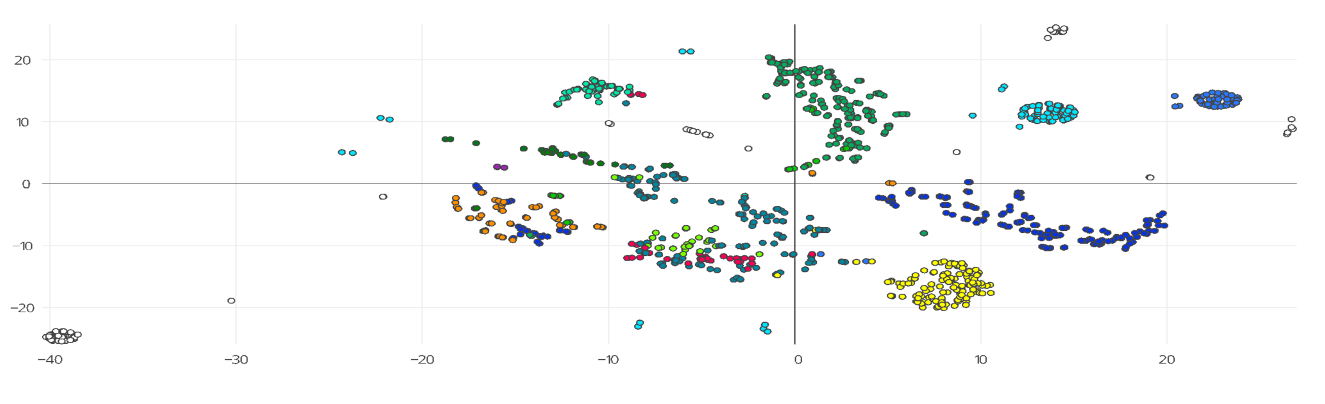
\includegraphics[width = 130mm, height=75mm]{stanf_lc_kmeans.png}
	\caption{Rappresentazione del sito \texttt{cs.stanford.edu}, clusterizzato con K-Means.}
	\label{lc_embText_km}
\end{figure}

Nonostante il dataset del grafo completo presenti un maggiore coefficiente di Silhouette, l'applicazione delle listehanno restituito risultati migliori. In questo caso hanno filtrato in modo consistente le pagine esplorate in quanto il DOM del sito includeva la maggior parte degli hyperlink in sezione nascoste, prevalentemente menù dropdown. Questo ha garantito una diversificazione marcata dei percorsi. Inoltre i risultati dell'analisi testuale si attestano al di sotto di quelli ottenuti attraverso l'URL embedding. 

Anche qui i cluster si sono formati prevalentemente con forma sferica, favorendo il K-Means sugli altri.

\subsubsection{\texttt{eecs.mit.edu}}

\begin{table}[H]
	\begin{tabular}{| l | c | c | c | c | c | c |}
	\hline
	\textbf{MIT}  & \textbf{Hom} & \textbf{Com} & \textbf{V-M}  & \textbf{ARI}  & \textbf{MI}  & \textbf{Silh} \\ [2ex] \hline
	\textbf{G-nc WT} & 0.1792 & 0.6729 & 0.2830 & 0.1762 & 0.1648 & // \\ [2ex]
	 \hline
	\textbf{G-nc FG} & 0.5769 & 0.5215 & 0.5478 & 0.5514 & 0.5119 & // \\ [2ex]
	 \hline	
	\textbf{G-lc WT} & 0.0856 & 0.5013 & 0.1462 & 0.0450 & 0.0664 & // \\ [2ex]
	 \hline	
	\textbf{G-lc FG} & 0.5617 & \textbf{0.7127} & \textbf{0.6282} & \textbf{0.6851} & \textbf{0.5497} & // \\ [2ex]
	\hline

	\textbf{E-nc dbscan} & 0.4097 & 0.4236 & 0.4164 & 0.3779 & 0.3869 & \textbf{0.3264}\\ [2ex]
	 \hline 
	\textbf{E-nc hdbscan} & 0.5834 & 0.4413 & 0.5025 & 0.5811 & 0.4231 & 0.3141\\ [2ex]
	 \hline
	\textbf{E-nc Kmeans} & 0.6422 & 0.5129 & 0.5703 & 0.5141 & 0.5011 & 0.3914\\ [2ex]
	 \hline	
	\textbf{E-lc dbscan} & 0.1727 & 0.5736 & 0.2655 & 0.1455 & 0.1550 & 0.1750\\ [2ex]
	\hline
	\textbf{E-lc hdbscan} & \textbf{0.7882} & 0.4456 & 0.5693 & 0.5217 & 0.4061 & 0.2288\\ [2ex]
	\hline
	\textbf{E-lc Kmeans} & 0.7165 & 0.5283 & 0.6081 & 0.3625 & 0.5146 & 0.2646\\ [2ex]
	\hline
	
	\textbf{T-nc dbscan} & 0.2071 & 0.1908 & 0.1986 & 0.1011 & 0.1759 & 0.1133\\ [2ex]
	 \hline 
	\textbf{T-nc hdbscan} & 0.2363 & 0.2679 & 0.2611 & 0.0918 & 0.2207 & 0.0845\\ [2ex]
	 \hline
	\textbf{T-nc Kmeans} & 0.4175 & 0.2381 & 0.3032 & 0.0917 & 0.2290 & 0.1958\\ [2ex]
	 \hline	
	\textbf{T-lc dbscan} & 0.3470 & 0.3466 & 0.3467 & 0.2071 & 0.3326 & 0.1180\\ [2ex]
	\hline
	\textbf{T-lc hdbscan} & 0.4402 & 0.4147 & 0.4271 & 0.2806 & 0.3995 & 0.1423\\ [2ex]
	\hline
	\textbf{T-lc Kmeans} & 0.5857 & 0.4198 & 0.4890 & 0.2597 & 0.4085 & 0.2296\\ [2ex]
	\hline
	
	\textbf{ET-nc hdbscan} & 0.5573 & 0.3748 & 0.4482 & 0.2845 & 0.3600 & 0.1607\\ [2ex]
	 \hline
	\textbf{ET-nc Kmeans} & 0.5505 & 0.4344 & 0.4856 & 0.2687 & 0.4252 & 0.1699\\ [2ex]
	 \hline	
	\textbf{ET-lc hdbscan} & 0.6076 & 0.4329 & 0.5056 & 0.1910 & 0.4181 & 0.1464\\ [2ex]
	\hline
	\textbf{ET-lc Kmeans} & 0.6679 & 0.5332 & 0.5930 & 0.3499 & 0.5235 & 0.2311\\ [2ex]
	\hline	
	
	\end{tabular}
	\caption{Risultati sperimentazione del grafo del sito \texttt{eecs.mit.edu}}
	\label{metricheMit}
\end{table}

\begin{figure}[ht!]
	\centering
	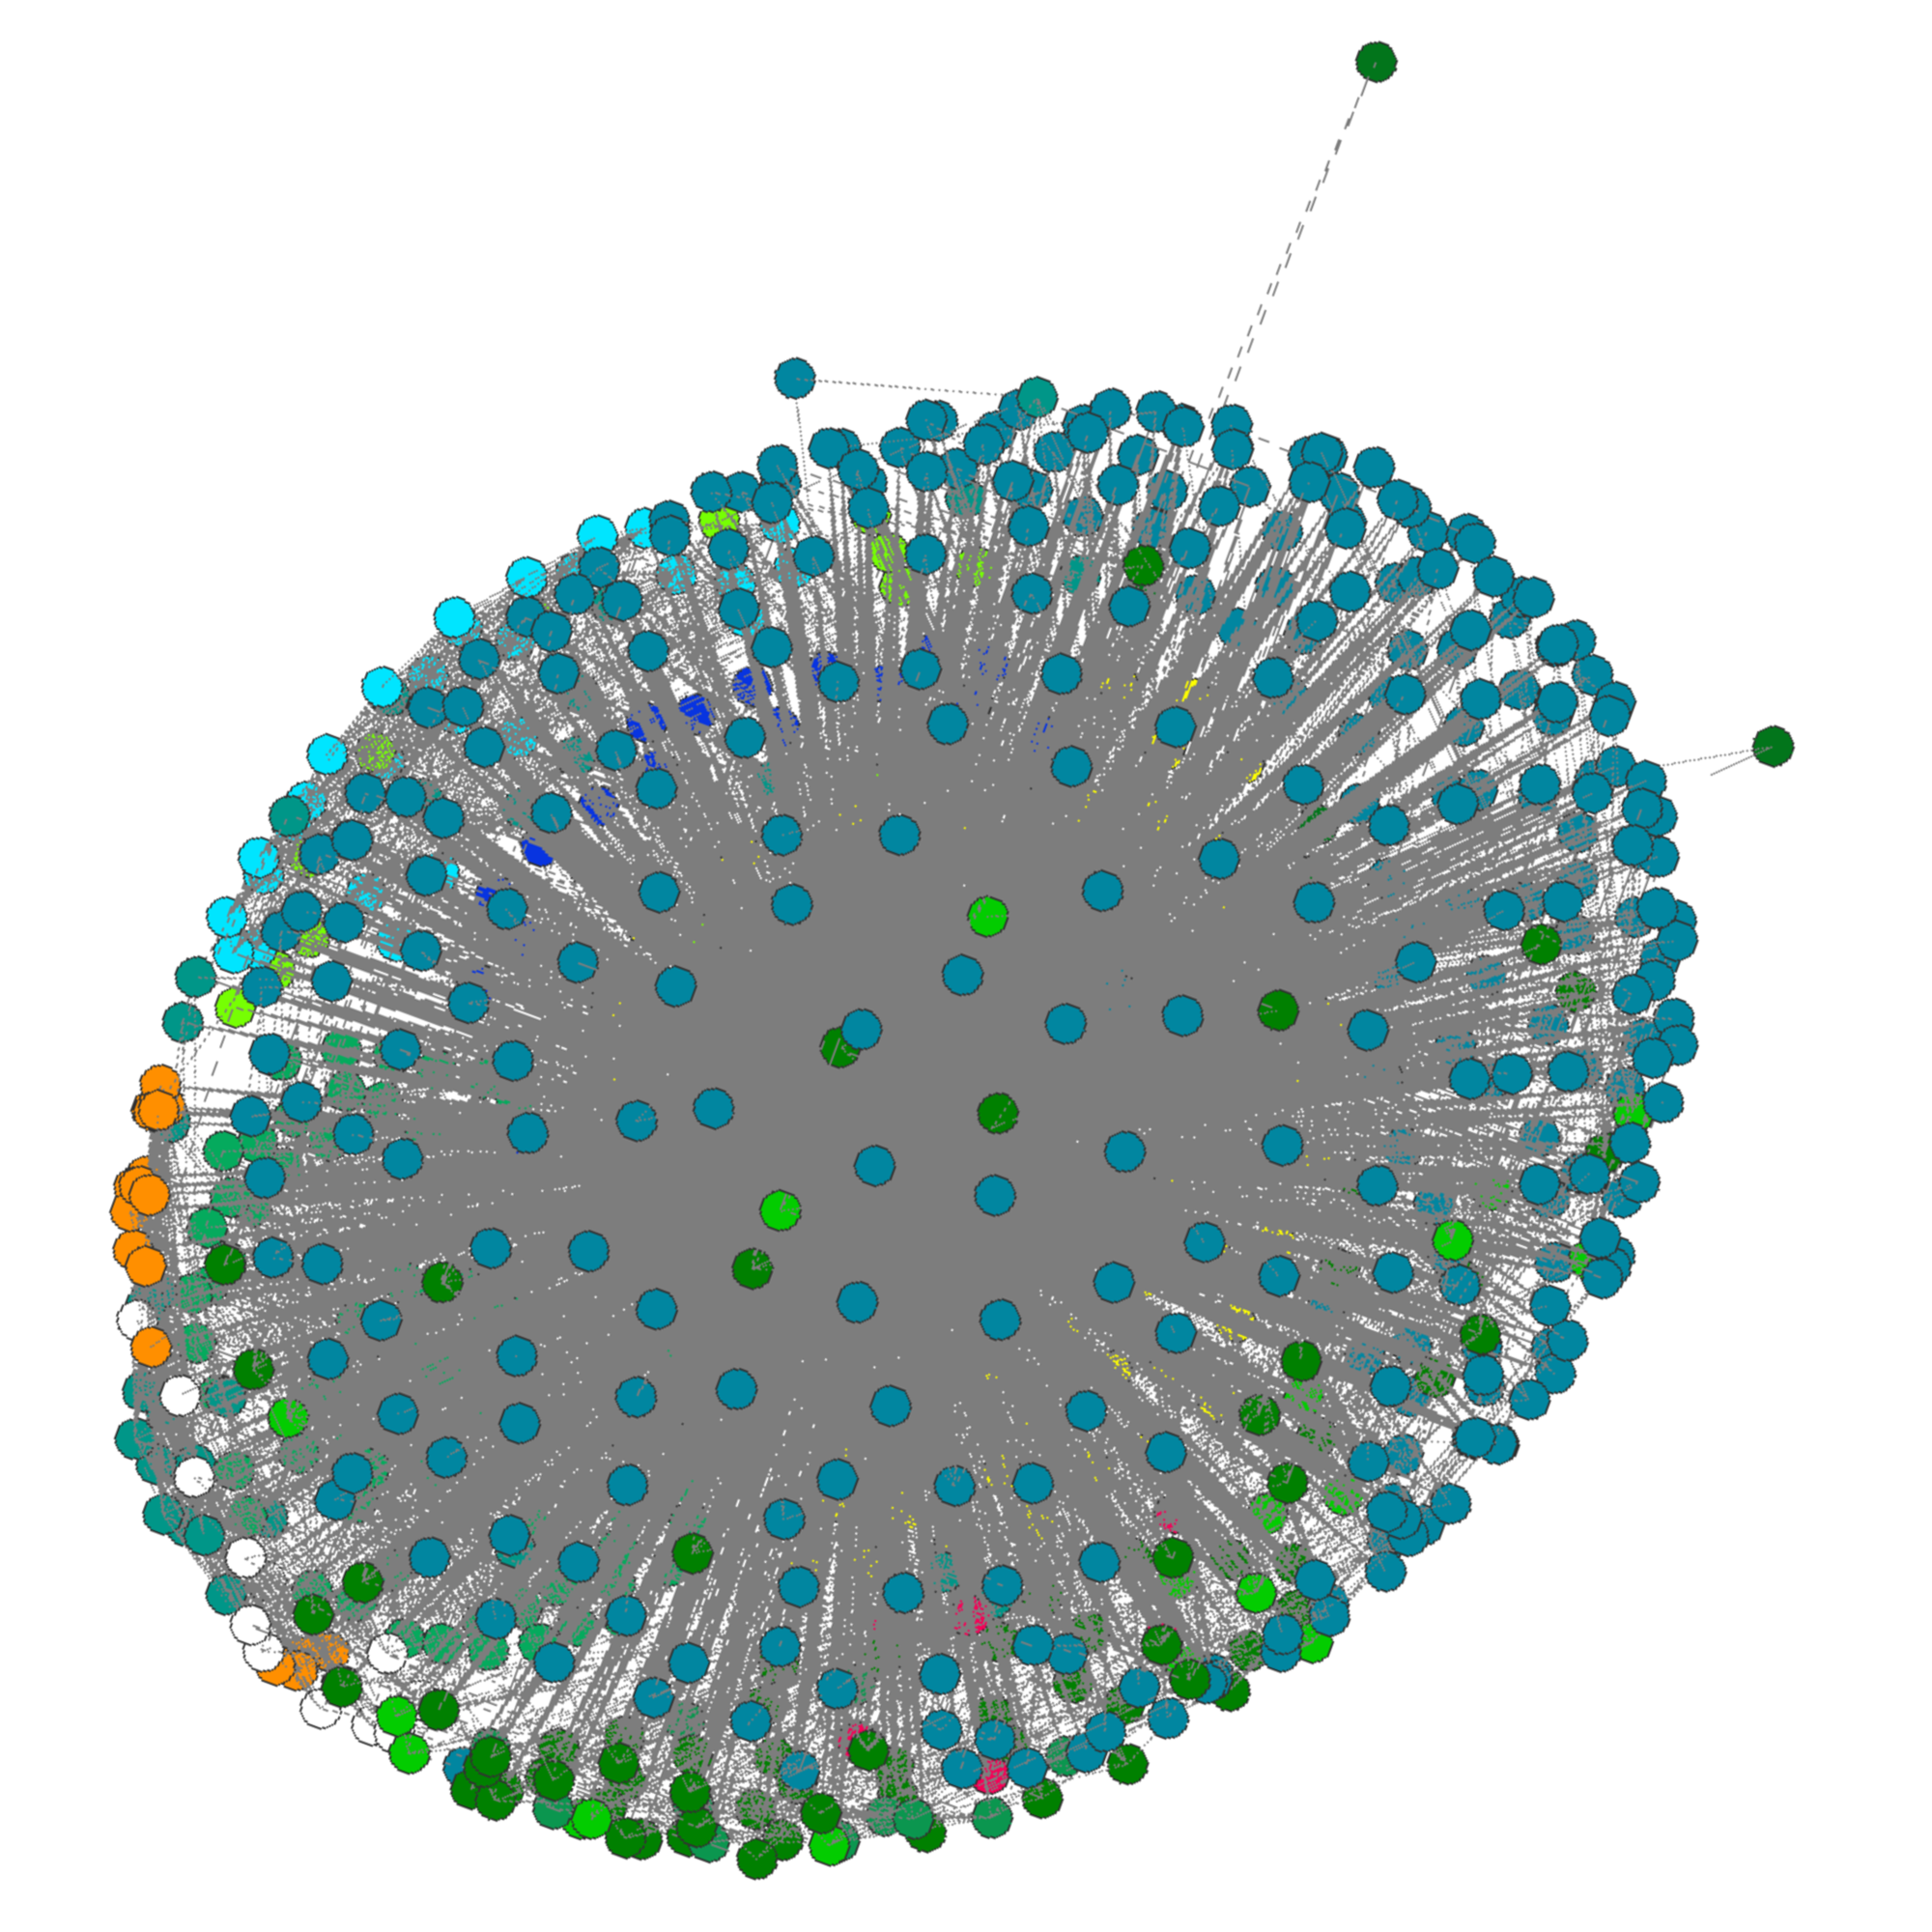
\includegraphics[width = 130mm]{mit_lc_fg.png}
	\caption{Rappresentazione del sito \texttt{eecs.mit.edu}, clusterizzato con Fastgreedy.}
	\label{lc_embText_km}
\end{figure}
In questo caso il partizionamento del grafo si è rivelato più efficace. L'embedding degli URL ha comunque restituito una omogeneità dei cluster maggiore. In questo caso i Random Walk, sia nell'algoritmo WalkTrap sul grafo, sia quelli utilizzati per apprendere rappresentazioni vettoriali, non sono riusciti a codificare abbastanza informazioni. La modularità del grafo, utilizzata in Fastgreedy, ha evidenziato una forte divisione fra le Community presenti. Questo è stato dovuto dalle maggiori connessioni tra le pagine all'interno dello stesso cluster, rispetto alle connessioni fra pagine di cluster diversi. Le liste hanno contribuito a filtrare i cammini percorribili.
\subsubsection{\texttt{cs.princeton.edu}}

\begin{table}[H]
	\begin{tabular}{| l | c | c | c | c | c | c |}
	\hline
	\textbf{Princeton}  & \textbf{Hom} & \textbf{Com} & \textbf{V-M}  & \textbf{ARI}  & \textbf{MI}  & \textbf{Silh} \\ [3ex] \hline
	\textbf{G-nc WT} & 0.0259 & 0.1568 & 0.0444 & -0.0221 & 0.0197 & // \\ [2ex]
	 \hline
	\textbf{G-nc FG} & 0.4900 & \textbf{0.5702} & 0.5270 & 0.4594 & 0.4848 & // \\ [2ex]
	 \hline	
	\textbf{G-lc WT} & 0.1543 & 0.2983 & 0.2034 & 0.1935 & 0.1375 & // \\ [2ex]
	 \hline	
	\textbf{G-lc FG} & 0.4230 & 0.3817 & 0.4013 & 0.2168 & 0.3686 & // \\ [2ex]
	\hline
	
	\textbf{E-nc dbscan} & 0.0955 & 0.2417 & 0.1369 & 0.0622 & 0.0886 & 0.2656\\ [2ex]
	 \hline 
	\textbf{E-nc hdbscan} & 0.2302 & 0.3292 & 0.2710 & 0.1651 & 0.2195 & 0.1687\\ [2ex]
	 \hline
	\textbf{E-nc Kmeans} & 0.4311 & 0.3637 & 0.3946 & 0.3404 & 0.3522 & 0.3877\\ [2ex]
	 \hline	
	\textbf{E-lc dbscan} & 0.5941 & 0.5696 & 0.5816 & 0.7706 & \textbf{0.5579} & 0.2269\\ [2ex]
	\hline
	\textbf{E-lc hdbscan} & 0.6531 & 0.5416 & \textbf{0.5922} & \textbf{0.7708} & 0.5275 & 0.1789\\ [2ex]
	\hline
	\textbf{E-lc Kmeans} & \textbf{0.7611} & 0.4448 & 0.5615 & 0.4571 & 0.4304 & 0.2282\\ [2ex]
	\hline
	
	\textbf{T-nc dbscan} & 0.4231 & 0.3935 & 0.4078 & 0.3441 & 0.3773 & 0.4627\\ [2ex]
	 \hline 
	\textbf{T-nc hdbscan} & 0.3385 & 0.3082 & 0.3227 & 0.2662 & 0.2941 & 0.3442\\ [2ex]
	 \hline
	\textbf{T-nc Kmeans} & 0.4402 & 0.3369 & 0.3817 & 0.3891 & 0.3313 & \textbf{0.5111}\\ [2ex]
	 \hline	
	\textbf{T-lc dbscan} & 0.3352 & 0.2267 & 0.2704 & 0.0513 & 0.1926 & 0.1077\\ [2ex]
	\hline
	\textbf{T-lc hdbscan} & 0.3099 & 0.2081 & 0.2490 & 0.1101 & 0.1772 & 0.1092\\ [2ex]
	\hline
	\textbf{T-lc Kmeans} & 0.6906 & 0.3715 & 0.4832 & 0.2795 & 0.3602 & 0.2115\\ [2ex]
	\hline
	
	\textbf{ET-nc hdbscan} & 0.1663 & 0.1963 & 0.1801 & -0.0134 & 0.1541 & 0.0379\\ [2ex]
	 \hline
	\textbf{ET-nc Kmeans} & 0.4006 & 0.3326 & 0.3634 & 0.2929 & 0.3223 & 0.1974\\ [2ex]
	 \hline	
	\textbf{ET-lc hdbscan} & 0.3024 & 0.3582 & 0.3279 & 0.1848 & 0.2913 & 0.0325\\ [2ex]
	\hline
	\textbf{ET-lc Kmeans} & 0.7387 & 0.3921 & 0.5122 & 0.3175 & 0.3782 & 0.1307\\ [2ex]
	\hline
	
	\end{tabular}
	\caption{Risultati sperimentazione del sito \texttt{cs.princeton.edu}}
	\label{metrichePrinc}
\end{table}

\begin{figure}[ht!]
	\centering
	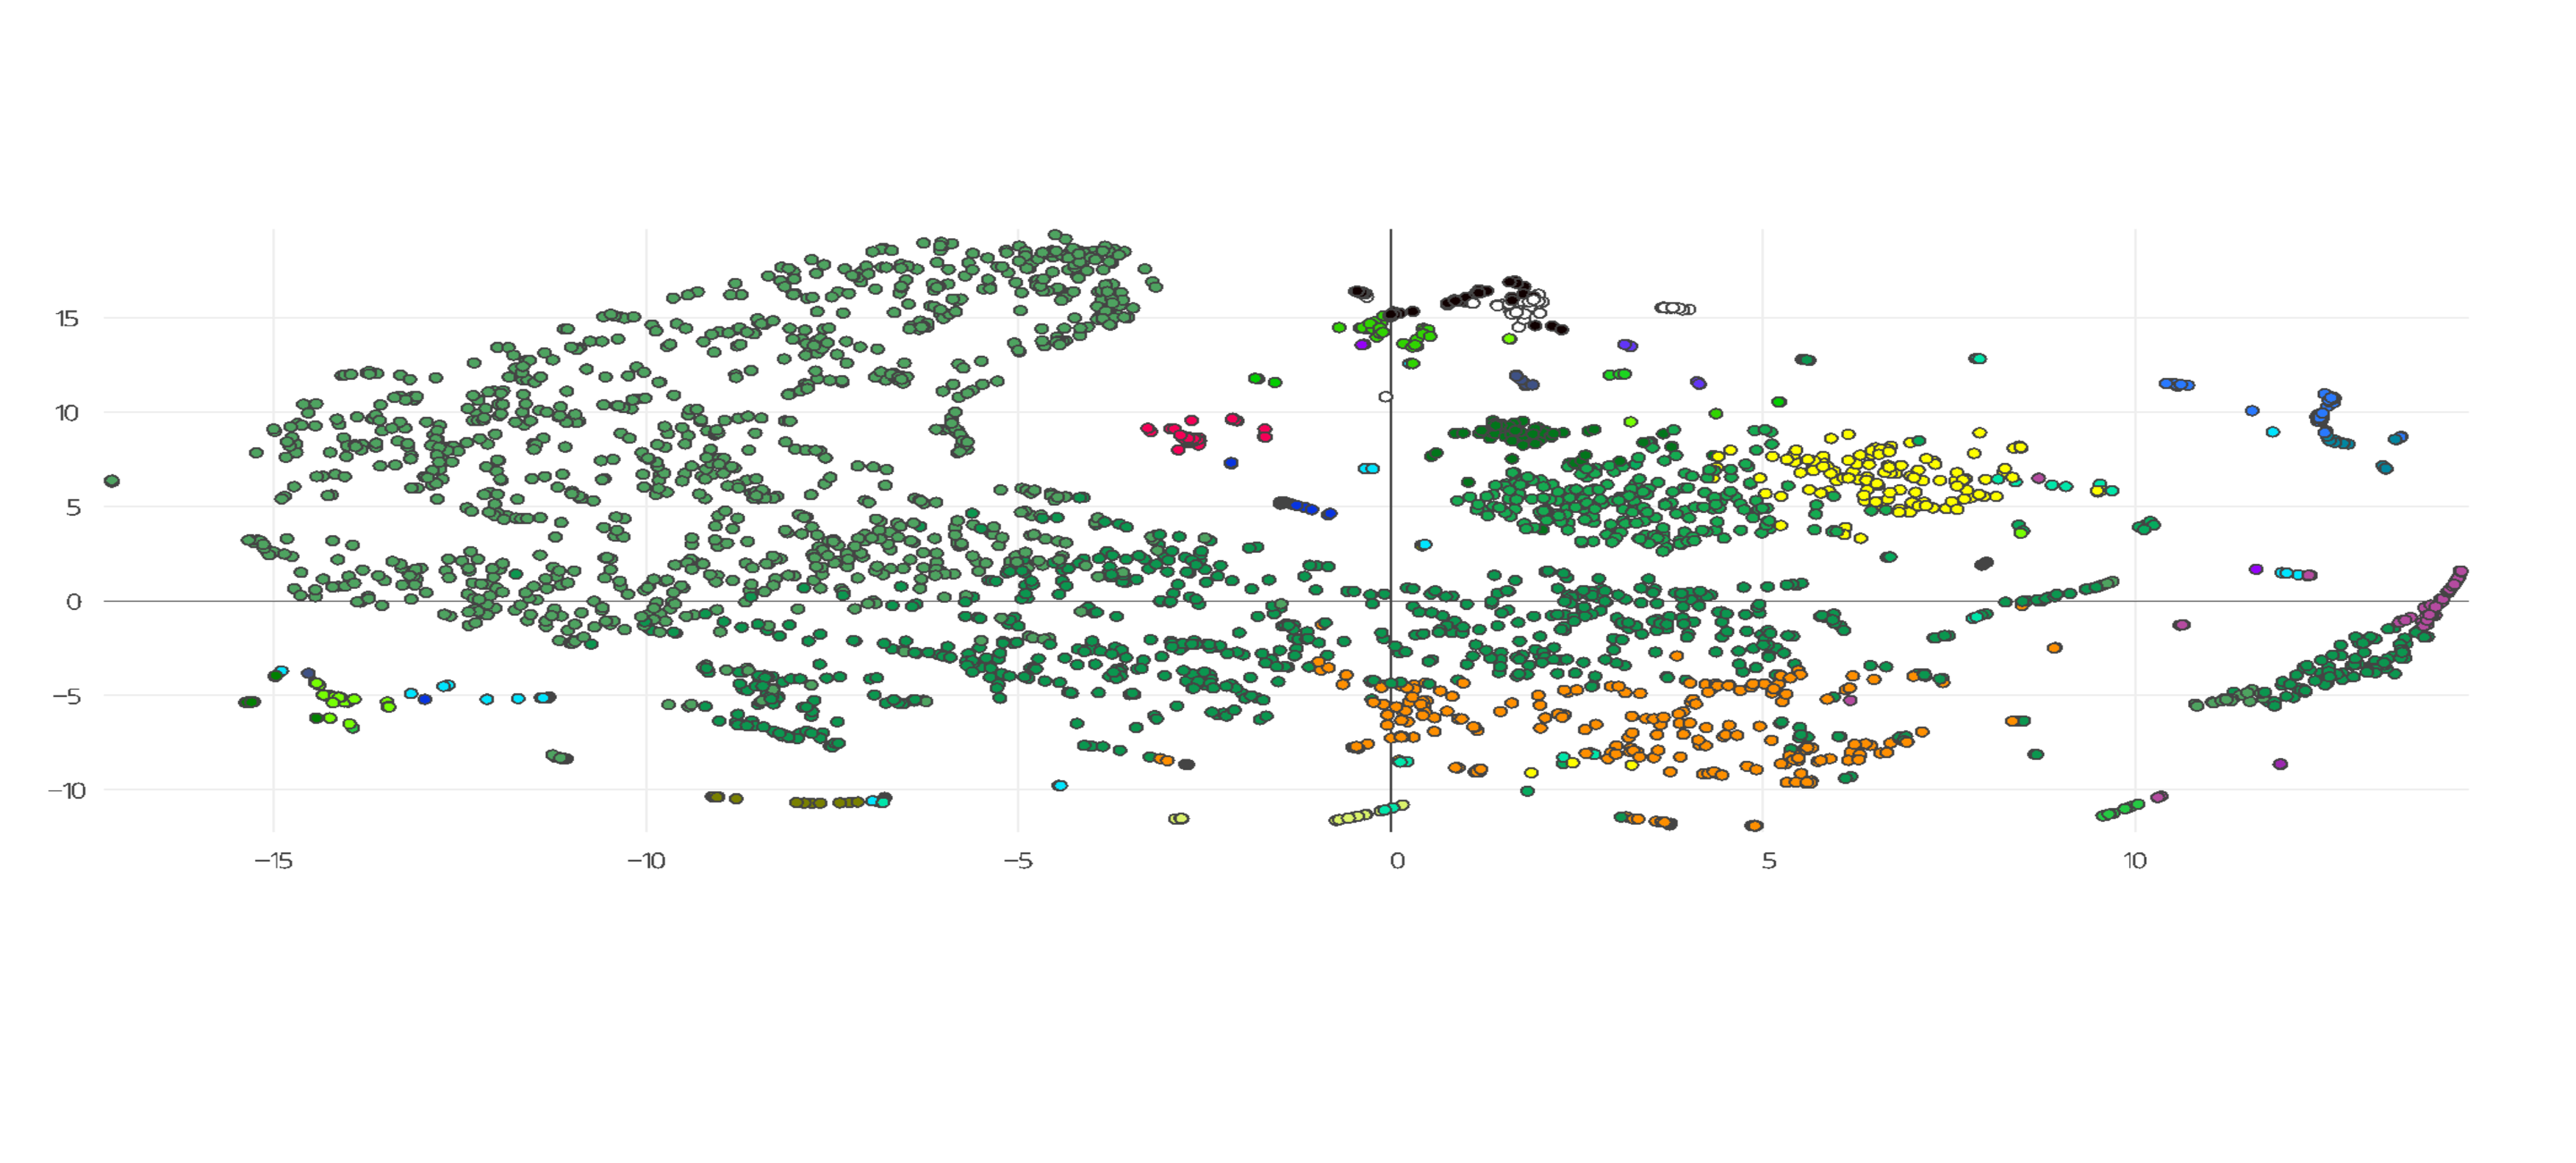
\includegraphics[width = 130mm, height=93mm]{prince_emb_lc_h.png}
	\caption{Rappresentazione del sito \texttt{cs.princeton.edu}, clusterizzato con Fastgreedy.}
	\label{lc_emb_h}
\end{figure}

I cluster generati dalle rappresentazioni vettoriali delle pagine hanno formato cluster densi. L'algoritmo HDBSCAN è riuscito a distinguere meglio le pagine presentano la più alta V-measure e Adjusted Random Index. Anche qui le liste hanno migliorato notevolmente i risultati ottenuti. 


\subsubsection{\texttt{cs.ox.ac.uk}}

\begin{table}[H]
	\begin{tabular}{| l | c | c | c | c | c | c |}
	\hline
	\textbf{Oxford}  & \textbf{Hom} & \textbf{Com} & \textbf{V-M}  & \textbf{ARI}  & \textbf{MI} & \textbf{Silh} \\ [2ex] \hline
	\textbf{G-nc WT} & 0.2264 & \textbf{0.8330} & 0.3560 & 0.1133 & 0.2149 & // \\ [2ex]
	 \hline
	\textbf{G-nc FG} & 0.4416 & 0.5005 & 0.4692 & 0.2617 & 0.4302 & // \\ [2ex]
	 \hline	
	\textbf{G-lc WT} & 0.1888 & 0.5069 & 0.2751 & 0.0034 & 0.1753 & // \\ [2ex]
	 \hline	
	\textbf{G-lc FG} & 0.4445 & 0.4444 & 0.4444 & 0.1758 & 0.4322 & // \\ [2ex]
	\hline

	\textbf{E-nc dbscan} & 0.2289 & 0.4673 & 0.3073 & 0.1777 & 0.2126 & 0.5214 \\ [2ex]
	 \hline 
	\textbf{E-nc hdbscan} & 0.2391 & 0.4616 & 0.3150 & 0.1811 & 0.2213 & \textbf{0.5241} \\ [2ex]
	 \hline
	\textbf{E-nc Kmeans} & 0.3966 & 0.4649 & 0.4281 & 0.2516 & 0.3746 & 0.3991 \\ [2ex]
	 \hline	
	\textbf{E-lc dbscan} & 0.2401 & 0.5187 & 0.3282 & 0.2619 & 0.2319 & 0.5037 \\ [2ex]
	\hline
	\textbf{E-lc hdbscan} & 0.3007 & 0.5382 & 0.3859 & \textbf{0.2965} & 0.2880 & 0.4503 \\ [2ex]
	\hline
	\textbf{E-lc Kmeans} & 0.4247 & 0.4010 & 0.4125 & 0.2630 & 0.3788 & 0.2372 \\ [2ex]
	\hline
	
	\textbf{T-nc dbscan} & 0.2014 & 0.5083 & 0.2885 & 0.0658 & 0.1813 & -0.1190 \\ [2ex]
	 \hline 
	\textbf{T-nc hdbscan} & 0.3421 & 0.4731 & 0.3971 & 0.1062 & 0.3260 & 0.0598 \\ [2ex]
	 \hline
	\textbf{T-nc Kmeans} & 0.7021 & 0.4976 & 0.5825 & 0.2714 & \textbf{0.4821} & 0.1555 \\ [2ex]
	 \hline	
	\textbf{T-lc dbscan} & 0.4961 & 0.4837 & 0.4898 & 0.2616 & 0.4689 & 0.1319 \\ [2ex]
	\hline
	\textbf{T-lc hdbscan} & 0.4613 & 0.4744 & 0.4677 & 0.1219 & 0.4418 & 0.0526 \\ [2ex]
	\hline
	\textbf{T-lc Kmeans} & \textbf{0.7314} & 0.4946 & \textbf{0.5901} & 0.2623 & 0.4813 & 0.1600 \\ [2ex]
	\hline
	
	\textbf{ET-nc hdbscan} & 0.1343 & 0.1762 & 0.1524 & -0.0357 & 0.1012 & -0.0826 \\ [2ex]
	 \hline
	\textbf{ET-nc Kmeans} & 0.3681 & 0.3052 & 0.3338 & 0.1337 & 0.2846 & 0.1322 \\ [2ex]
	 \hline	
	\textbf{ET-lc hdbscan} & 0.1537 & 0.1741 & 0.1632 & -0.0383 & 0.1248 & -0.0319 \\ [2ex]
	\hline
	\textbf{ET-lc Kmeans} & 0.3869 & 0.2836 & 0.3273 & 0.1277 & 0.2638 & 0.1386 \\ [2ex]
	\hline
	\end{tabular}
	\caption{Risultati sperimentazione del sito \texttt{cs.ox.ac.uk}}
	\label{metricheOx}
\end{table}

L'analisi testuale ha sorpassato di gran lunge le altre rappresentazioni. Nel sito dell'università di Oxford, le pagine si sono rivelate consistenti tra loro e con gli argomenti trattati mentre l'analisi della componente connessa del sito non è stata sufficiente per riuscire ad estrarre le informazioni desiderate. I topic dell'università inglese si sono rivelati la componente più informativa.

\color{red}
QUESTA PARTE METTILA NELLA PARTE DI DISCUSSIONE DEI RISULTATI.


\color{black}
\subsection{Community Detection}
%Sono state applicate metodologie derivanti dalla teoria dei grafi per l'estrazione di strutture connesse all'interno del grafo web. Questo può essere utile nella individuazione di community all'interno di grafi come ad esempio social network. Sono stati comunque effettuati test utilizzando la rappresentazione a grafo per confrontare al meglio i risultati globali ottenuti.I grafi utilizzati rappresentano le due diverse operazioni di estrazione di collegamenti effettuate. La prima contiene tutti i collegamenti presenti all'interno di una pagina e mostrerà quindi più archi. La seconda estrae solamente gli hyperlink dalle liste. L'analisi del grafo considera unicamente le relazioni che intercorrono fra le pagine web e tralascia informazioni riguardanti il contenuto. Dalle metriche rilevate risulta in tabella \ref{metricheGraphIll}, risulta che il partizionamento del grafo web non riesce a dividere al meglio i cluster.
 
\begin{figure}[htb]
	\centering
	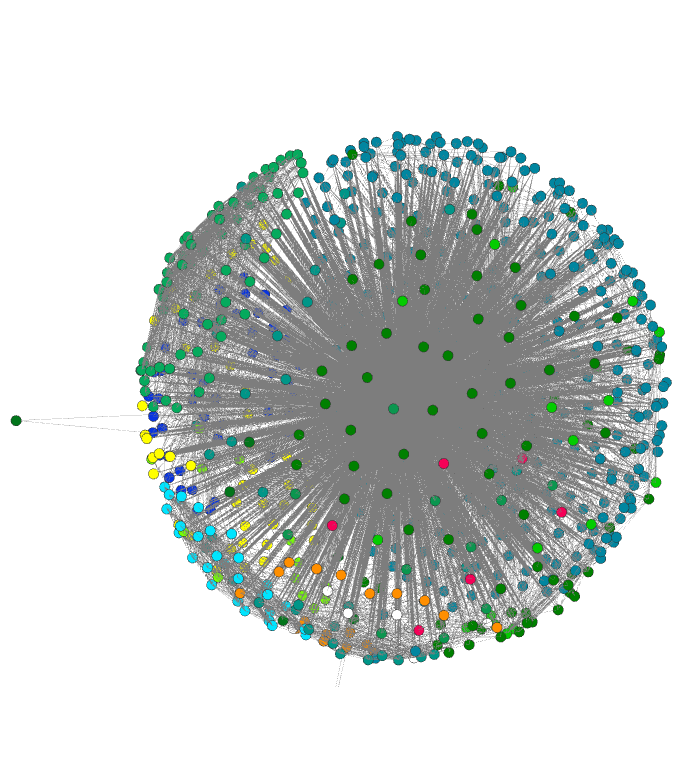
\includegraphics[width = 100mm]{nc_groundtruth.png}
	\caption{Grafo del sito \texttt{cs.illinois.edu} etichettato manualmente.}
	\label{nc_groundtruth}
\end{figure}

\paragraph{\texttt{cs.illinois.edu}}L'algoritmo \textit{Fastgreedy} non richiede parametri specifici ma è stato tagliato il dendrogramma ad altezza $15$, il numero di cluster nella operazione di raggruppamento manuale. Ugualmente per \textit{WalkTrap}, che però necessitava della lunghezza dei Random Walk da effettuare. I risultati migliori sono stati osservati con percorsi di lunghezza $3$.
\begin{table}[H]
	\begin{tabular}{| l | c | c | c | c | c |}
	\hline
	\textbf{G - Illinois}  & \textbf{Homog} & \textbf{Compl} & \textbf{V-Measure}  & \textbf{ARI}  & \textbf{MI} \\ [3ex] \hline
	\textbf{nc WalkTrap} & 0.6471 & 0.6585 & 0.6527 & 0.4363 & 0.6281\\ [3ex]
	 \hline
	\textbf{nc Fastgreedy} & 0.5518 & 0.8563 & 0.6711 & 0.5764 & 0.5354\\ [3ex]
	 \hline	
	\textbf{lc WalkTrap} & 0.5093 & 0.4892 & 0.4991 & 0.2762 & 0.4722\\ [3ex]
	 \hline	
	\textbf{lc Fastgreedy} & 0.5522 & 0.6035 & 0.5767 & 0.3656 & 0.5382\\ [3ex]
	\hline
	\end{tabular}
	\caption{Risultati sperimentazione di partizionamento del grafo del sito \texttt{cs.illinois.edu}}
	\label{metricheGraphIll}
\end{table}
 
\paragraph{\texttt{cs.stanford.edu}} Il grafo del sito presenta $1458$ nodi e $99686$ archi. Il dendrogramma restituito dall'algoritmo \textit{Fastgreedy} è stato troncato ad altezza $10$. Anche qui la scelta è ricaduta su Random Wlak di lunghezza $3$ per l'algoritmo \textit{WalkTrap}.

\begin{table}[H]
	\begin{tabular}{| l | c | c | c | c | c |}
	\hline
	\textbf{G - Stanford}  & \textbf{Homog} & \textbf{Compl} & \textbf{V-Measure}  & \textbf{ARI}  & \textbf{MI} \\ [3ex] 
	\hline
	\textbf{nc WalkTrap} & 0.1628 & 0.3967 & 0.2308 & 0.1127 & 0.1340 \\[3ex]
	 \hline
	\textbf{nc Fastgreedy} & 0.3568 & 0.3894 & 0.3724 & 0.2439 & 0.3357 \\[3ex]
	 \hline	
	\textbf{lc WalkTrap} & 0.3087 & 0.6314 & 0.4146 & 0.0502 & 0.1911 \\[3ex]
	 \hline	
	\textbf{lc Fastgreedy} & 0.4854 & 0.6740 & 0.5644 & 0.2999 & 0.3892\\ [3ex]
	\hline
	\end{tabular}
	\caption{Risultati sperimentazione di partizionamento del grafo del sito \texttt{cs.stanford.edu}}
	\label{metricheGraphStanf}
\end{table}
 
\paragraph{\texttt{eecs.mit.edu}} Il grafo del sito presenta $1745$ nodi e $63937$ archi. L'algoritmo \textit{Fastgreedy} ha costruito un dendrogramma che è stato tagliato ad altezza $15$, il numero di cluster nella operazione di raggruppamento manuale. Ugualmente per \textit{WalkTrap}, che però necessitava della lunghezza dei Random Walk da effettuare. I risultati migliori sono stati osservati con percorsi di lunghezza $3$.

\begin{table}[H]
	\begin{tabular}{| l | c | c | c | c | c |}
	\hline
	\textbf{G - MIT}  & \textbf{Homog} & \textbf{Compl} & \textbf{V-Measure}  & \textbf{ARI}  & \textbf{MI} \\ [3ex] \hline
	\textbf{nc WalkTrap} & 0.1792 & 0.6729 & 0.2830 & 0.1762 & 0.1648\\ [3ex]
	 \hline
	\textbf{nc Fastgreedy} & 0.5769 & 0.5215 & 0.5478 & 0.5514 & 0.5119\\ [3ex]
	 \hline	
	\textbf{lc WalkTrap} & 0.0856 & 0.5013 & 0.1462 & 0.0450 & 0.0664\\ [3ex]
	 \hline	
	\textbf{lc Fastgreedy} & 0.5617 & 0.7127 & 0.6282 & 0.6851 & 0.5497\\ [3ex]
	\hline
	\end{tabular}
	\caption{Risultati sperimentazione di partizionamento del grafo del sito \texttt{eecs.mit.edu}}
	\label{metricheGraphMit}
\end{table}

\paragraph{\texttt{cs.princeton.edu}} Il grafo del sito presenta $16378$ nodi e $206985$ archi. L'algoritmo \textit{Fastgreedy} ha costruito un dendrogramma che è stato tagliato ad altezza $20$, il numero di cluster nella operazione di raggruppamento manuale. Ugualmente per \textit{WalkTrap}, che però necessitava della lunghezza dei Random Walk da effettuare. I risultati migliori sono stati osservati con percorsi di lunghezza $4$.

\begin{table}[H]
	\begin{tabular}{| l | c | c | c | c | c |}
	\hline
	\textbf{G - Princeton}  & \textbf{Homog} & \textbf{Compl} & \textbf{V-Measure}  & \textbf{ARI}  & \textbf{MI} \\ [3ex] \hline
	\textbf{nc WalkTrap} & 0.0259 & 0.1568 & 0.0444 & -0.0221 & 0.0197\\ [3ex]
	 \hline
	\textbf{nc Fastgreedy} & 0.4900 & 0.5702 & 0.5270 & 0.4594 & 0.4848\\ [3ex]
	 \hline	
	\textbf{lc WalkTrap} & 0.1543 & 0.2983 & 0.2034 & 0.1935 & 0.1375\\ [3ex]
	 \hline	
	\textbf{lc Fastgreedy} & 0.4230 & 0.3817 & 0.4013 & 0.2168 & 0.3686\\ [3ex]
	\hline
	\end{tabular}
	\caption{Risultati sperimentazione di partizionamento del grafo del sito \texttt{cs.princeton.edu}}
	\label{metricheGraphPrinc}
\end{table}

\paragraph{\texttt{cs.ox.ac.uk}} Il grafo del sito presenta $4183$ nodi e $27954$ archi. L'algoritmo \textit{Fastgreedy} ha costruito un dendrogramma che è stato tagliato ad altezza $20$, il numero di cluster nella operazione di raggruppamento manuale. Ugualmente per \textit{WalkTrap}, che però necessitava della lunghezza dei Random Walk da effettuare. I risultati migliori sono stati osservati con percorsi di lunghezza $4$.

\begin{table}[H]
	\begin{tabular}{| l | c | c | c | c | c |}
	\hline
	\textbf{G - Oxford}  & \textbf{Homog} & \textbf{Compl} & \textbf{V-Measure}  & \textbf{ARI}  & \textbf{MI} \\ [3ex] \hline
	\textbf{nc WalkTrap} & 0.2264 & 0.8330 & 0.3560 & 0.1133 & 0.2149 \\ [3ex]
	 \hline
	\textbf{nc Fastgreedy} & 0.4416 & 0.5005 & 0.4692 & 0.2617 & 0.4302 \\ [3ex]
	 \hline	
	\textbf{lc WalkTrap} & 0.1888 & 0.5069 & 0.2751 & 0.0034 & 0.1753 \\ [3ex]
	 \hline	
	\textbf{lc Fastgreedy} & 0.4445 & 0.4444 & 0.4444 & 0.1758 & 0.4322 \\ [3ex]
	\hline
	\end{tabular}
	\caption{Risultati sperimentazione di partizionamento del grafo del sito \texttt{cs.ox.ac.uk}}
	\label{metricheGraphOx}
\end{table}


\subsection{URL Embedding}
Considerando i Random Walk generati sul grafo come frasi, è possibile applicare algoritmi di Word Embedding per raggruppare le pagine sulla base del contesto in cui appaiono, ovvero le pagine che più verosimilmente appariranno insieme nelle sequenze.
\\
Le squenze di Random Walk sono state usate per apprendere rappresentazioni vettoriali delle pagine Web. La fase di URL embedding è stata effetuata utilizzando l'algoritmo Word2vec, \cite{gensim} (esaminato in \ref{word2vec}) modificando alcuni parametri e lasciando invariato altri.
\\
I parametri personalizzati sono:
\begin{itemize}
\item \textbf{min-count}: tutte le parole (o URL) con frequenza di occorrenza minore i questo valore vengono ignorate.
\item \textbf{window} rappresenta la distanza massima tra l'URL corrente e quello predetto all'interno di una frase.
\item \textbf{negative} Nella fase di embedding di una URL, viene calcolato il rapporto tra la similarità del contesto con la parola e la sommatoria di tutte le similarità tra la parola e gli altri contesti. Più precisamente:
\begin{equation}
\frac{v_c \cdot v_w}{\sum\limits_{c \in C} v_c \cdot v_w}
\end{equation}
Questa operazione può essere molto lenta. Per accelerare il processo possono venir scelti $n$ contesti casuali da confrontare. Questo parametro, se maggiore di $0$, rappresenta il numero di vettori da confrontare.
\item \textbf{sg} definisce l'algoritmo di apprendimento, di default viene usato \textit{CBOW}, mentre se impostato a $1$ utilizza \textit{skip-gram} \cite{Mikolov13}. Per lo scopo della sperimentazione si imposterà questo valore a  CBOW.
\end{itemize}
I migliori risultati sono stati osservati con:

\paragraph{\texttt{cs.illinois.edu}} è stata impostato un \textit{min-count} pari a $1$, \textit{window} con valore $5$ ed è stato utilizzato \textit{skip-gram} con $5$ \textit{negative} sampling. Gli algoritmi testati sono stati: DBSCAN con $\epsilon = 0.9$ ed \textit{min-samples}$ = 4$; HDBSCAN con \textit{min-cluster-size}$=6$; K-Means con numero di cluster pari a $15$. 

\begin{table}[H]
	\begin{tabular}{| l | c | c | c | c | c | c |}
	\hline
	\textbf{E - Illinois}  & \textbf{Homog} & \textbf{Compl} & \textbf{V-Meas}  & \textbf{ARI}  & \textbf{MI}  & \textbf{Silh} \\ [3ex] 		\hline
	\textbf{nc dbscan} & 0.5553 & 0.6579 & 0.6023 & 0.4487 & 0.5234 & 0.2588\\ [3ex]
	 \hline 
	\textbf{nc hdbscan} & 0.5759 & 0.6720 & 0.6203 & 0.5282 & 0.5525 & 0.2573\\ [3ex]
	 \hline
	\textbf{nc Kmeans} & 0.8238 & 0.7575 & 0.7892 & 0.7883 & 0.7423 & 0.3131\\ [3ex]
	 \hline	
	\textbf{lc dbscan} & 0.4163 & 0.5922 & 0.4889 & 0.2250 & 0.3935 & 0.1320\\ [3ex]
	\hline
	\textbf{lc hdbscan} & 0.4760 & 0.5067 & 0.4908 & 0.2275 & 0.4515 & 0.1054\\ [3ex]
	\hline
	\textbf{lc Kmeans} & 0.8095 & 0.6593 & 0.7267 & 0.6189 & 0.6473 & 0.2281\\ [3ex]
	\hline
	\end{tabular}
	\caption{Risultati sperimentazione di URL embedding del sito \texttt{cs.illinois.edu}}
	\label{metricheEmbedIll}
\end{table}

\paragraph{\texttt{cs.stanford.edu}} è stata impostato un \textit{min-count} pari a $1$, \textit{window} con valore $5$ ed è stato utilizzato \textit{skip-gram} con $5$ \textit{negative} sampling. Gli algoritmi testati sono stati: DBSCAN con $\epsilon = 0.9$ ed \textit{min-samples}$ = 7$; HDBSCAN con \textit{min-cluster-size}$=10$; K-Means con numero di cluster pari a $15$. Per il dataset delle liste: DBSCAN con $\epsilon = 1.6$ ed \textit{min-samples}$ = 3$; HDBSCAN con \textit{min-cluster-size}$=5$; K-Means con numero di cluster pari a $15$.

\begin{table}[H]
	\begin{tabular}{| l | c | c | c | c | c | c |}
	\hline
	\textbf{E - Stanford}  & \textbf{Homog} & \textbf{Compl} & \textbf{V-Meas}  & \textbf{ARI}  & \textbf{MI}  & \textbf{Silh} \\ [3ex] \hline
	\textbf{nc dbscan} & 0.3453 & 0.4031 & 0.3720 & 0.2577 & 0.3252 & 0.4058\\ [3ex]
	 \hline 
	\textbf{nc hdbscan} & 0.4720 & 0.4418 & 0.4564 & 0.3094 & 0.4210 & 0.4030\\ [3ex]
	 \hline
	\textbf{nc Kmeans} & 0.3810 & 0.3844 & 0.3827 & 0.2276 & 0.3574 & 0.5659\\ [3ex]
	 \hline	
	\textbf{lc dbscan} & 0.4830 & 0.5798 & 0.5270 & 0.0976 & 0.3363 & 0.0938\\ [3ex]
	\hline
	\textbf{lc hdbscan} & 0.6506 & 0.6299 & 0.6353 & 0.2466 & 0.5014 & 0.1762\\ [3ex]
	\hline
	\textbf{lc Kmeans} & 0.5853 & 0.6838 & 0.6308 & 0.2423 & 0.4786 & 0.2513\\ [3ex]
	\hline
	\end{tabular}
	\caption{Risultati sperimentazione di URL embedding del sito \texttt{cs.stanford.edu}}
	\label{metricheEmbedStanf}
\end{table}

\paragraph{\texttt{eecs.mit.edu}} è stata impostato un \textit{min-count} pari a $1$, \textit{window} con valore $5$ ed è stato utilizzato \textit{skip-gram} con $5$ \textit{negative} sampling. Gli algoritmi testati sono stati: DBSCAN con $\epsilon = 1.0$ ed \textit{min-samples}$ = 10$; HDBSCAN con \textit{min-cluster-size}$=10$; K-Means con numero di cluster pari a $10$. Per il dataset delle liste: DBSCAN con $\epsilon = 1.5$ ed \textit{min-samples}$ = 5$; HDBSCAN con \textit{min-cluster-size}$=13$; K-Means con numero di cluster pari a $10$.

\begin{table}[H]
	\begin{tabular}{| l | c | c | c | c | c | c |}
	\hline
	\textbf{E - MIT}  & \textbf{Homog} & \textbf{Compl} & \textbf{V-Meas}  & \textbf{ARI}  & \textbf{MI}  & \textbf{Silh} \\ [3ex] \hline
	\textbf{nc dbscan} & 0.4097 & 0.4236 & 0.4164 & 0.3779 & 0.3869 & 0.3264\\ [3ex]
	 \hline 
	\textbf{nc hdbscan} & 0.5834 & 0.4413 & 0.5025 & 0.5811 & 0.4231 & 0.3141\\ [3ex]
	 \hline
	\textbf{nc Kmeans} & 0.6422 & 0.5129 & 0.5703 & 0.5141 & 0.5011 & 0.3914\\ [3ex]
	 \hline	
	\textbf{lc dbscan} & 0.1727 & 0.5736 & 0.2655 & 0.1455 & 0.1550 & 0.1750\\ [3ex]
	\hline
	\textbf{lc hdbscan} & 0.7882 & 0.4456 & 0.5693 & 0.5217 & 0.4061 & 0.2288\\ [3ex]
	\hline
	\textbf{lc Kmeans} & 0.7165 & 0.5283 & 0.6081 & 0.3625 & 0.5146 & 0.2646\\ [3ex]
	\hline
	\end{tabular}
	\caption{Risultati sperimentazione di URL embedding del sito \texttt{eecs.mit.edu}}
	\label{metricheEmbedMit}
\end{table}

\paragraph{\texttt{cs.princeton.edu}} è stata impostato un \textit{min-count} pari a $1$, \textit{window} con valore $5$ ed è stato utilizzato \textit{skip-gram} con $5$ \textit{negative} sampling. Gli algoritmi testati sono stati: DBSCAN con $\epsilon = 0.8$ ed \textit{min-samples}$ = 7$; HDBSCAN con \textit{min-cluster-size}$=10$; K-Means con numero di cluster pari a $30$. Per il dataset delle liste: DBSCAN con $\epsilon = 0.7$ ed \textit{min-samples}$ = 5$; HDBSCAN con \textit{min-cluster-size}$=8$; K-Means con numero di cluster pari a $25$.

\begin{table}[H]
	\begin{tabular}{| l | c | c | c | c | c | c |}
	\hline
	\textbf{E - Princeton}  & \textbf{Homog} & \textbf{Compl} & \textbf{V-Meas}  & \textbf{ARI}  & \textbf{MI}  & \textbf{Silh} \\ [3ex] \hline
	\textbf{nc dbscan} & 0.0955 & 0.2417 & 0.1369 & 0.0622 & 0.0886 & 0.2656\\ [3ex]
	 \hline 
	\textbf{nc hdbscan} & 0.2302 & 0.3292 & 0.2710 & 0.1651 & 0.2195 & 0.1687\\ [3ex]
	 \hline
	\textbf{nc Kmeans} & 0.4311 & 0.3637 & 0.3946 & 0.3404 & 0.3522 & 0.3877\\ [3ex]
	 \hline	
	\textbf{lc dbscan} & 0.5941 & 0.5696 & 0.5816 & 0.7706 & 0.5579 & 0.2269\\ [3ex]
	\hline
	\textbf{lc hdbscan} & 0.6531 & 0.5416 & 0.5922 & 0.7708 & 0.5275 & 0.1789\\ [3ex]
	\hline
	\textbf{lc Kmeans} & 0.7611 & 0.4448 & 0.5615 & 0.4571 & 0.4304 & 0.2282\\ [3ex]
	\hline
	\end{tabular}
	\caption{Risultati sperimentazione di URL embedding del sito \texttt{cs.princeton.edu}}
	\label{metricheEmbedPrinc}
\end{table}

\paragraph{\texttt{cs.ox.ac.uk}} è stata impostato un \textit{min-count} pari a $1$, \textit{window} con valore $5$ ed è stato utilizzato \textit{skip-gram} con $5$ \textit{negative} sampling. Gli algoritmi testati sono stati: DBSCAN con $\epsilon = 0.8$ ed \textit{min-samples}$ = 7$; HDBSCAN con \textit{min-cluster-size}$=10$; K-Means con numero di cluster pari a $30$. Per il dataset delle liste: DBSCAN con $\epsilon = 0.7$ ed \textit{min-samples}$ = 5$; HDBSCAN con \textit{min-cluster-size}$=8$; K-Means con numero di cluster pari a $25$.


\begin{table}[H]
	\begin{tabular}{| l | c | c | c | c | c | c |}
	\hline
	\textbf{E - Oxford}  & \textbf{Homog} & \textbf{Compl} & \textbf{V-Meas}  & \textbf{ARI}  & \textbf{MI}  & \textbf{Silh} \\ [3ex] \hline
	\textbf{nc dbscan} & 0.2289 & 0.4673 & 0.3073 & 0.1777 & 0.2126 & 0.5214 \\ [3ex]
	 \hline 
	\textbf{nc hdbscan} & 0.2391 & 0.4616 & 0.3150 & 0.1811 & 0.2213 & 0.5241 \\ [3ex]
	 \hline
	\textbf{nc Kmeans} & 0.3966 & 0.4649 & 0.4281 & 0.2516 & 0.3746 & 0.3991 \\ [3ex]
	 \hline	
	\textbf{lc dbscan} & 0.2401 & 0.5187 & 0.3282 & 0.2619 & 0.2319 & 0.5037 \\ [3ex]
	\hline
	\textbf{lc hdbscan} & 0.3007 & 0.5382 & 0.3859 & 0.2965 & 0.288052 & 0.4503 \\ [3ex]
	\hline
	\textbf{lc Kmeans} & 0.4247 & 0.4010 & 0.4125 & 0.2630 & 0.3788 & 0.2372 \\ [3ex]
	\hline
	\end{tabular}
	\caption{Risultati sperimentazione di URL embedding del sito \texttt{cs.ox.ac.uk}}
	\label{metricheEmbedOx}
\end{table}

\subsection{Text Mining}
Sono state utilizzate tecniche di Text Mining per il clustering basato sul contenuto testuale. I contenuti all'interno di uno stesso sito web avranno una struttura e termini comuni, differenziandosi al variare dell'argomento trattato. La struttura gerarchica di un sito web organizza solitamente le pagine in sezioni simili. Questa metodologia tuttavia, considera solo l'informazione testuale, assumendo che i termini all'interno del sito web siano indipendenti l'uno dall'altro così come i documenti, ignorando le relazioni interdipendenti tra questi. Il web si discosta dall'analisi classica dei documenti proprio per le relazioni che intercorrono tra le pagine, tuttavia l'analisi testuale rimane molto importante.
\\
Nella fase di sperimentazione è stata utilizzata una rappresentazione vettoriale della frequenza dei termini all'interno dell'insieme delle pagine web, calcolata con la tecnica della \textit{frequency–inverse document frequency} (tf-idf).

I parametri personalizzati per la costruzione dell matrice documenti-termini con funzione di peso \textit{idf} sono stati:
\begin{itemize}
\item \textbf{max-df}: questo valore rappresenta la massima frequenza, all'interno dei documenti, che un termine può avere per essere utilizzato nella matrice tf-idf. Se un termine appare molte volte nel corpus, molto probabilmente avrà poco significato.
\item \textbf{min-df}: indica il numero minimo di documenti in cui un termine dovrà apparire per essere considerato.
\item \textbf{ngram-range}: vengono presi in considerazioni gli n-grammi di lunghezza compresa nell'intervallo specificato in questo parametro. Un n-gramma è una sottosequenza  di $n$ elementi di un'altra.
\end{itemize}

I risultati mostrati sono stati ottenuti nel seguente modo:
\paragraph{\texttt{cs.illinois.edu}}
Sul dataset del sito, costituito da $728$ pagine e $433$ termini, il corpus è stato ripulito delle stopword, stemmatizzato ed è stato impostato il \textit{max-df} all'80\%, il \textit{min-df} a $0.1$ e sono stati considerati solo uni-grammi, bi-grammi e tri-grammi. Se i termini appaiono in più dell'80\% dei documenti, probabilmente avrà poco significato, lo stesso se appare troppe poche volte. Gli algoritmi testati sono stati: DBSCAN con $\epsilon = 0.9$ ed \textit{min-samples}$ = 4$; HDBSCAN con \textit{min-cluster-size}$=4$; K-Means con numero di cluster pari a $15$. \\Sul Dataset costruito estraendo le liste: DBSCAN con $\epsilon = 0.7$ ed \textit{min-samples}$ = 4$; HDBSCAN con \textit{min-cluster-size}$=7$; K-Means con numero di cluster pari a $15$. 

\begin{table}[H]
	\begin{tabular}{| l | c | c | c | c | c | c |}
	\hline
	\textbf{T - Illinois}  & \textbf{Homog} & \textbf{Compl} & \textbf{V-Meas}  & \textbf{ARI}  & \textbf{MI}  & \textbf{Silh} \\ [3ex] \hline
	\textbf{nc dbscan} & 0.5601 & 0.5962 & 0.5776 & 0.4078 & 0.5346 & 0.1242\\ [3ex]
	 \hline 
	\textbf{nc hdbscan} & 0.5152 & 0.6029 & 0.5556 & 0.3862 & 0.4858 & 0.0881\\ [3ex]
	 \hline
	\textbf{nc Kmeans} & 0.7619 & 0.5814 & 0.6596 & 0.3184 & 0.5586 & 0.1767\\ [3ex]
	 \hline	
	\textbf{lc dbscan} & 0.5710 & 0.7042 & 0.6306 & 0.5197 & 0.5566 & 0.1406\\ [3ex]
	\hline
	\textbf{lc hdbscan} & 0.4501 & 0.5104 & 0.4783 & 0.1938 & 0.4297 & 0.1018\\ [3ex]
	\hline
	\textbf{lc Kmeans} & 0.8061 & 0.5892 & 0.6808 & 0.4296 & 0.5748 & 0.2002\\ [3ex]
	\hline
	\end{tabular}
	\caption{Risultati sperimentazione di Text Mining del sito \texttt{cs.illinois.edu}}
	\label{metricheTextIll}
\end{table}

\paragraph{\texttt{cs.stanford.edu}}
Sul dataset del sito, costituito da $1458$ pagine e $843$ termini, il corpus è stato ripulito delle stopword, stemmatizzato ed è stato impostato il \textit{max-df} all'80\%, il \textit{min-df} a $0.1$ e sono stati considerati solo uni-grammi, bi-grammi e tri-grammi. Se i termini appaiono in più dell'80\% dei documenti, probabilmente avrà poco significato, lo stesso se appare troppe poche volte. Gli algoritmi testati sono stati: DBSCAN con $\epsilon = 0.3$ ed \textit{min-samples}$ = 5$; HDBSCAN con \textit{min-cluster-size}$=15$; K-Means con numero di cluster pari a $15$. \\Sul Dataset costruito estraendo le liste: DBSCAN con $\epsilon = 0.5$ ed \textit{min-samples}$ = 3$; HDBSCAN con \textit{min-cluster-size}$=5$; K-Means con numero di cluster pari a $15$. 


\begin{table}[H]
	\begin{tabular}{| l | c | c | c | c | c | c |}
	\hline
	\textbf{T - Stanford}  & \textbf{Homog} & \textbf{Compl} & \textbf{V-Meas}  & \textbf{ARI}  & \textbf{MI}  & \textbf{Silh} \\ [3ex] \hline
	\textbf{nc dbscan} & 0.2584 & 0.3435 & 0.2949 & 0.0208 & 0.2403 & 0.0981\\ [3ex]
	 \hline 
	\textbf{nc hdbscan} & 0.3015 & 0.2784 & 0.2895 & 0.0089 & 0.2521 & 0.0916\\ [3ex]
	 \hline
	\textbf{nc Kmeans} & 0.6014 & 0.4652 & 0.5246 & 0.2639 & 0.4489 & 0.2704\\ [3ex]
	 \hline	
	\textbf{lc dbscan} & 0.0876 & 0.3924 & 0.1432 & 0.0102 & 0.0327 & -0.1188\\ [3ex]
	\hline
	\textbf{lc hdbscan} & 0.1827 & 0.3802 & 0.2468 & 0.0687 & 0.1326 & 0.0841\\ [3ex]
	\hline
	\textbf{lc Kmeans} & 0.5436 & 0.5726 & 0.5577 & 0.2167 & 0.4157 & 0.1732\\ [3ex]
	\hline
	\end{tabular}
	\caption{Risultati sperimentazione di Text Mining del sito \texttt{cs.stanford.edu}}
	\label{metricheTextStanf}
\end{table}

\paragraph{\texttt{eecs.mit.edu}}
Sul dataset del sito, costituito da $1745$ pagine e $354$ termini, il corpus è stato ripulito delle stopword, stemmatizzato ed è stato impostato il \textit{max-df} all'80\%, il \textit{min-df} a $0.1$ e sono stati considerati solo uni-grammi, bi-grammi e tri-grammi. Se i termini appaiono in più dell'80\% dei documenti, probabilmente avrà poco significato, lo stesso se appare troppe poche volte. Gli algoritmi testati sono stati: DBSCAN con $\epsilon = 0.9$ ed \textit{min-samples}$ = 9$; HDBSCAN con \textit{min-cluster-size}$=15$; K-Means con numero di cluster pari a $10$. \\Sul Dataset costruito estraendo le liste: DBSCAN con $\epsilon = 0.9$ ed \textit{min-samples}$ = 6$; HDBSCAN con \textit{min-cluster-size}$=9$; K-Means con numero di cluster pari a $10$. 

\begin{table}[H]
	\begin{tabular}{| l | c | c | c | c | c | c |}
	\hline
	\textbf{T - MIT}  & \textbf{Homog} & \textbf{Compl} & \textbf{V-Meas}  & \textbf{ARI}  & \textbf{MI}  & \textbf{Silh} \\ [3ex] \hline
	\textbf{nc dbscan} & 0.2071 & 0.1908 & 0.1986 & 0.1011 & 0.1759 & 0.1133\\ [3ex]
	 \hline 
	\textbf{nc hdbscan} & 0.2363 & 0.2679 & 0.2611 & 0.0918 & 0.2207 & 0.0845\\ [3ex]
	 \hline
	\textbf{nc Kmeans} & 0.4175 & 0.2381 & 0.3032 & 0.0917 & 0.2290 & 0.1958\\ [3ex]
	 \hline	
	\textbf{lc dbscan} & 0.3470 & 0.3466 & 0.3467 & 0.2071 & 0.3326 & 0.1180\\ [3ex]
	\hline
	\textbf{lc hdbscan} & 0.4402 & 0.4147 & 0.4271 & 0.2806 & 0.3995 & 0.1423\\ [3ex]
	\hline
	\textbf{lc Kmeans} & 0.5857 & 0.4198 & 0.4890 & 0.2597 & 0.4085 & 0.2296\\ [3ex]
	\hline
	\end{tabular}
	\caption{Risultati sperimentazione di Text Mining del sito \texttt{eecs.mit.edu}}
	\label{metricheTextMit}
\end{table}

\paragraph{\texttt{cs.princeton.edu}}
Sul dataset del sito, costituito da $16378$ pagine e $470$ termini, il corpus è stato ripulito delle stopword, stemmatizzato ed è stato impostato il \textit{max-df} all'80\%, il \textit{min-df} a $0.1$ e sono stati considerati solo uni-grammi, bi-grammi e tri-grammi. Se i termini appaiono in più dell'80\% dei documenti, probabilmente avrà poco significato, lo stesso se appare troppe poche volte. Gli algoritmi testati sono stati: DBSCAN con $\epsilon = 0.3$ ed \textit{min-samples}$ = 5$; HDBSCAN con \textit{min-cluster-size}$=15$; K-Means con numero di cluster pari a $10$. \\Sul Dataset costruito estraendo le liste: DBSCAN con $\epsilon = 0.9$ ed \textit{min-samples}$ = 6$; HDBSCAN con \textit{min-cluster-size}$=15$; K-Means con numero di cluster pari a $25$.  

\begin{table}[H]
	\begin{tabular}{| l | c | c | c | c | c | c |}
	\hline
	\textbf{T - Princeton}  & \textbf{Homog} & \textbf{Compl} & \textbf{V-Meas}  & \textbf{ARI}  & \textbf{MI}  & \textbf{Silh} \\ [3ex] \hline
	\textbf{nc dbscan} & 0.4231 & 0.3935 & 0.4078 & 0.3441 & 0.3773 & 0.4627\\ [3ex]
	 \hline 
	\textbf{nc hdbscan} & 0.3385 & 0.3082 & 0.3227 & 0.2662 & 0.2941 & 0.3442\\ [3ex]
	 \hline
	\textbf{nc Kmeans} & 0.4402 & 0.3369 & 0.3817 & 0.3891 & 0.3313 & 0.5111\\ [3ex]
	 \hline	
	\textbf{lc dbscan} & 0.3352 & 0.2267 & 0.2704 & 0.0513 & 0.1926 & 0.1077\\ [3ex]
	\hline
	\textbf{lc hdbscan} & 0.3099 & 0.2081 & 0.2490 & 0.1101 & 0.1772 & 0.1092\\ [3ex]
	\hline
	\textbf{lc Kmeans} & 0.6906 & 0.3715 & 0.4832 & 0.2795 & 0.3602 & 0.2115\\ [3ex]
	\hline
	\end{tabular}
	\caption{Risultati sperimentazione di Text Mining del sito \texttt{cs.princeton.edu}}
	\label{metricheTextPrinc}
\end{table}

\paragraph{\texttt{cs.ox.ac.uk}}
Sul dataset del sito, costituito da $3951$ pagine e $363$ termini, il corpus è stato ripulito delle stopword, stemmatizzato ed è stato impostato il \textit{max-df} all'80\%, il \textit{min-df} a $0.1$ e sono stati considerati solo uni-grammi, bi-grammi e tri-grammi. Se i termini appaiono in più dell'80\% dei documenti, probabilmente avrà poco significato, lo stesso se appare troppe poche volte. Gli algoritmi testati sono stati: DBSCAN con $\epsilon = 0.3$ ed \textit{min-samples}$ = 5$; HDBSCAN con \textit{min-cluster-size}$=15$; K-Means con numero di cluster pari a $10$. \\Sul Dataset costruito estraendo le liste: DBSCAN con $\epsilon = 0.7$ ed \textit{min-samples}$ = 7$; HDBSCAN con \textit{min-cluster-size}$=7$; K-Means con numero di cluster pari a $25$. 

\begin{table}[H]
	\begin{tabular}{| l | c | c | c | c | c | c |}
	\hline
	\textbf{T - Oxford}  & \textbf{Homog} & \textbf{Compl} & \textbf{V-Meas}  & \textbf{ARI}  & \textbf{MI}  & \textbf{Silh} \\ [3ex] \hline
	\textbf{nc dbscan} & 0.2014 & 0.5083 & 0.2885 & 0.0658 & 0.1813 & -0.1190 \\ [3ex]
	 \hline 
	\textbf{nc hdbscan} & 0.3421 & 0.4731 & 0.3971 & 0.1062 & 0.3260 & 0.0598 \\ [3ex]
	 \hline
	\textbf{nc Kmeans} & 0.7021 & 0.4976 & 0.5825 & 0.2714 & 0.4821 & 0.1555 \\ [3ex]
	 \hline	
	\textbf{lc dbscan} & 0.4961 & 0.4837 & 0.4898 & 0.2616 & 0.4689 & 0.1319 \\ [3ex]
	\hline
	\textbf{lc hdbscan} & 0.4613 & 0.4744 & 0.4677 & 0.1219 & 0.4418 & 0.0526 \\ [3ex]
	\hline
	\textbf{lc Kmeans} & 0.7314 & 0.4946 & 0.5901 & 0.2623 & 0.4813 & 0.1600 \\ [3ex]
	\hline
	\end{tabular}
	\caption{Risultati sperimentazione di Text Mining del sito \texttt{cs.ox.ac.uk}}
	\label{metricheTextOx}
\end{table}



\subsection{Embedding e Text Mining}
Sono stati quindi considerati come un unico vettore. Il vantaggio di associare entrambe le relazioni in uno spazio vettoriale offre il vantaggio usare la stessa rappresentazione e quindi di unire i vettori derivanti dagli algoritmi di Word Embedding con quelli derivanti dall'analisi di contenuto testuale. 
\\
Così facendo è possibile dare più importanza ad una tipologia di informazione piuttosto che ad un altra, andando a modificare il rapporto tra le dimensioni dei vettori.


\paragraph{\texttt{cs.illinois.edu}} I vettori di word2vec sono stati generati di dimensione $48$, mentre i vettori-riga documenti sono stati ridotti con \textit{TruncateSVD} a dimensione $50$. Gli algoritmi testati sono stati: HDBSCAN con \textit{min-cluster-size}$=7$; K-Means con numero di cluster pari a $15$. 


\begin{table}[H]
	\begin{tabular}{| l | c | c | c | c | c | c |}
	\hline
	\textbf{ET - Illinois}  & \textbf{Homog} & \textbf{Compl} & \textbf{V-Meas}  & \textbf{ARI}  & \textbf{MI}  & \textbf{Silh} \\ [3ex] \hline
	\textbf{nc hdbscan} & 0.7327 & 0.7534 & 0.7429 & 0.7204 & 0.7186 & 0.2070\\ [3ex]
	 \hline 
	\textbf{nc Kmeans} & 0.8812 & 0.8069 & 0.8424 & 0.8299 & 0.7949 & 0.3198\\ [3ex]
	 \hline
	\textbf{lc hdbscan} & 0.6541 & 0.6129 & 0.6328 & 0.3249 & 0.5992 & 0.1203\\ [3ex]
	\hline
	\textbf{lc Kmeans} & 0.8548 & 0.6885 & 0.7627 & 0.6488 & 0.6773 & 0.2573\\ [3ex]
	\hline
	\end{tabular}
	\caption{Risultati sperimentazione di Text-Embedding del sito \texttt{cs.illinois.edu}}
	\label{metricheTextEmbedIll}
\end{table}

\paragraph{\texttt{cs.stanford.edu}} I vettori di word2vec sono stati generati di dimensione $48$, mentre i vettori-riga documenti sono stati ridotti con \textit{TruncateSVD} a dimensione $50$. Gli algoritmi testati sono stati: HDBSCAN con \textit{min-cluster-size}$=10$; K-Means con numero di cluster pari a $15$. 


\begin{table}[H]
	\begin{tabular}{| l | c | c | c | c | c | c |}
	\hline
	\textbf{ET - Stanford}  & \textbf{Homog} & \textbf{Compl} & \textbf{V-Meas}  & \textbf{ARI}  & \textbf{MI}  & \textbf{Silh} \\ [3ex] 
	\hline
	\textbf{nc hdbscan} & 0.3495 & 0.5272 & 0.4203 & 0.3335 & 0.3307 & 0.3469\\ [3ex]
	 \hline
	\textbf{nc Kmeans} & 0.3490 & 0.3629 & 0.3558 & 0.2061 & 0.3238 & 0.4336\\ [3ex]
	 \hline	
	\textbf{lc hdbscan} & 0.2343 & 0.7045 & 0.3517 & 0.1012 & 0.2033 & 0.2342\\ [3ex]
	\hline
	\textbf{lc Kmeans} & 0.7508 & 0.7422 & 0.7465 & 0.5123 & 0.6656 & 0.2375\\ [3ex]
	\hline
	\end{tabular}
	\caption{Risultati sperimentazione di Text-Embedding del sito \texttt{cs.stanford.edu}}
	\label{metricheTextEmbedStanf}
\end{table}

\paragraph{\texttt{eecs.mit.edu}} I vettori di word2vec sono stati generati di dimensione $48$, mentre i vettori-riga documenti sono stati ridotti con \textit{TruncateSVD} a dimensione $50$. Gli algoritmi testati sono stati: HDBSCAN con \textit{min-cluster-size}$=14$; K-Means con numero di cluster pari a $10$. 


\begin{table}[H]
	\begin{tabular}{| l | c | c | c | c | c | c |}
	\hline
	\textbf{ET - MIT}  & \textbf{Homog} & \textbf{Compl} & \textbf{V-Meas}  & \textbf{ARI}  & \textbf{MI}  & \textbf{Silh} \\ [3ex] 
	\hline
	\textbf{nc hdbscan} & 0.5573 & 0.3748 & 0.4482 & 0.2845 & 0.3600 & 0.1607\\ [3ex]
	 \hline
	\textbf{nc Kmeans} & 0.5505 & 0.4344 & 0.4856 & 0.2687 & 0.4252 & 0.1699\\ [3ex]
	 \hline	
	\textbf{lc hdbscan} & 0.6076 & 0.4329 & 0.5056 & 0.1910 & 0.4181 & 0.1464\\ [3ex]
	\hline
	\textbf{lc Kmeans} & 0.6679 & 0.5332 & 0.5930 & 0.3499 & 0.5235 & 0.2311\\ [3ex]
	\hline
	\end{tabular}
	\caption{Risultati sperimentazione di Text-Embedding del sito \texttt{eecs.mit.edu}}
	\label{metricheTextEmbedMit}
\end{table}

\paragraph{\texttt{cs.princeton.edu}} I vettori di word2vec sono stati generati di dimensione $48$, mentre i vettori-riga documenti sono stati ridotti con \textit{TruncateSVD} a dimensione $50$. Gli algoritmi testati sono stati: HDBSCAN con \textit{min-cluster-size}$=14$; K-Means con numero di cluster pari a $10$. 


\begin{table}[H]
	\begin{tabular}{| l | c | c | c | c | c | c |}
	\hline
	\textbf{ET - Princeton}  & \textbf{Homog} & \textbf{Compl} & \textbf{V-Meas}  & \textbf{ARI}  & \textbf{MI}  & \textbf{Silh} \\ [3ex] 
	\hline
	\textbf{nc hdbscan} & 0.1663 & 0.1963 & 0.1801 & -0.0134 & 0.1541 & 0.0379\\ [3ex]
	 \hline
	\textbf{nc Kmeans} & 0.4006 & 0.3326 & 0.3634 & 0.2929 & 0.3223 & 0.1974\\ [3ex]
	 \hline	
	\textbf{lc hdbscan} & 0.3024 & 0.3582 & 0.3279 & 0.1848 & 0.2913 & 0.0325\\ [3ex]
	\hline
	\textbf{lc Kmeans} & 0.7387 & 0.3921 & 0.5122 & 0.3175 & 0.3782 & 0.1307\\ [3ex]
	\hline
	\end{tabular}
	\caption{Risultati sperimentazione di Text-Embedding del sito \texttt{cs.princeton.edu}}
	\label{metricheTextEmbedPrinc}
\end{table}

\paragraph{\texttt{cs.ox.ac.uk}} I vettori di word2vec sono stati generati di dimensione $48$, mentre i vettori-riga documenti sono stati ridotti con \textit{TruncateSVD} a dimensione $50$. Gli algoritmi testati sono stati: HDBSCAN con \textit{min-cluster-size}$=14$; K-Means con numero di cluster pari a $10$. 


\begin{table}[H]
	\begin{tabular}{| l | c | c | c | c | c | c |}
	\hline
	\textbf{ET - Oxford}  & \textbf{Homog} & \textbf{Compl} & \textbf{V-Meas}  & \textbf{ARI}  & \textbf{MI}  & \textbf{Silh} \\ [3ex] 
	\hline
	\textbf{nc hdbscan} & 0.1343 & 0.1762 & 0.1524 & -0.0357 & 0.1012 & -0.0826 \\ [3ex]
	 \hline
	\textbf{nc Kmeans} & 0.3681 & 0.3052 & 0.3338 & 0.1337 & 0.2846 & 0.1322 \\ [3ex]
	 \hline	
	\textbf{lc hdbscan} & 0.1537 & 0.1741 & 0.1632 & -0.0383 & 0.1248 & -0.0319 \\ [3ex]
	\hline
	\textbf{lc Kmeans} & 0.3869 & 0.2836 & 0.3273 & 0.1277 & 0.2638 & 0.1386 \\ [3ex]
	\hline
	\end{tabular}
	\caption{Risultati sperimentazione di Text-Embedding del sito \texttt{cs.ox.ac.uk}}
	\label{metricheTextEmbedOx}
\end{table}

\subsection{Analisi dei risultati}
Il processo di crawling è stato svolto su $3$ siti, sui quali sono state generate sequenze di $2$ tipi diversi, ossia Random Walk senza vincoli e Random Walk con i vincoli delle liste. Su di esse sono state poi effettuate $4$ metodologie diverse: grafo, Word Embedding, Text Mining e Word Embedding \& Text Mining. Per ogni metodologia, inoltre, sono stati usati $3$ algoritmi di apprendimento diversi, ovvero K-Means, HDBSCAN e DBSCAN. Infine, su ogni algoritmo sono state ricavate $6$ metriche. In tutto sono $432$ valori. 
\\\\
Di seguito sono riportati i risultati più interessanti per una migliore comprensione.

\textbf{K-Means nc - cs.illinois.edu}
\begin{table}[H]
	\begin{tabular}{| l | c | c | c | c | c | c |}
	\hline
	\textbf{Type}  & \textbf{Homog} & \textbf{Compl} & \textbf{V-Meas}  & \textbf{ARI}  & \textbf{MI}  & \textbf{Silh} \\ [3ex] \hline
	\textbf{Embedding} & 0.5553 & 0.6579 & 0.6023 & 0.4487 & 0.5234 & 0.2588\\ [3ex]
	 \hline 
	\textbf{Text Mining} & 0.5759 & 0.6720 & 0.6203 & 0.5282 & 0.5525 & 0.2573\\ [3ex]
	 \hline
	\textbf{Emb + Text} & 0.8238 & 0.7575 & 0.7892 & 0.7883 & 0.7423 & 0.3131\\ [3ex]
	 \hline
	\end{tabular}
	\caption{Risultati sperimentazione raggruppati per algoritmo K-Means sul sito \texttt{cs.illinois.edu}}
	\label{metricheTextEmbedKmeansNcIll}
\end{table}

In questo caso la combinazione delle due informazioni ha portato un miglioramento complessivo del clustering. Nel terzo caso si è verificato un miglioramento in media di $22.0$\% rispetto al primo, e di $18.8$\% rispetto al secondo.

\textbf{K-Means lc - cs.stanford.edu}
\begin{table}[H]
	\begin{tabular}{| l | c | c | c | c | c | c |}
	\hline
	\textbf{Type}  & \textbf{Homog} & \textbf{Compl} & \textbf{V-Meas}  & \textbf{ARI}  & \textbf{MI}  & \textbf{Silh} \\ [3ex] \hline
	\textbf{Embedding} & 0.5853 & 0.6838 & 0.6308 & 0.2423 & 0.4786 & 0.2513\\ [3ex]
	 \hline 
	\textbf{Text Mining} & 0.5857 & 0.4198 & 0.4890 & 0.2597 & 0.4085 & 0.2296\\ [3ex]
	 \hline
	\textbf{Emb + Text} & 0.7508 & 0.7422 & 0.7465 & 0.5123 & 0.6656 & 0.2375\\ [3ex]
	 \hline
	\end{tabular}
	\caption{Risultati sperimentazione raggruppati per algoritmo K-Means sul sito \texttt{ecs.mit.edu}}
	\label{metricheTextEmbedKmeansLcStanford}
\end{table}

Anche in questo caso l'utilizzo combinato di Text Mining e Word Embedding ha portato miglioramento. In media di $16$\% rispetto all'Embedding e di $21.2$\% rispetto al Text Mining. 

\textbf{K-Means lc - eecs.mit.edu}
\begin{table}[H]
	\begin{tabular}{| l | c | c | c | c | c | c |}
	\hline
	\textbf{Type}  & \textbf{Homog} & \textbf{Compl} & \textbf{V-Meas}  & \textbf{ARI}  & \textbf{MI}  & \textbf{Silh} \\ [3ex] \hline
	\textbf{Embedding} & 0.7165 & 0.5283 & 0.6081 & 0.3625 & 0.5146 & 0.2646\\ [3ex]
	 \hline 
	\textbf{Text Mining} & 0.5436 & 0.5726 & 0.5577 & 0.2167 & 0.4157 & 0.1732\\ [3ex]
	 \hline
	\textbf{Emb + Text} & 0.6679 & 0.5332 & 0.5930 & 0.3499 & 0.5235 & 0.2311\\ [3ex]
	 \hline
	\end{tabular}
	\caption{Risultati sperimentazione raggruppati per algoritmo K-Means sul sito \texttt{ecs.mit.edu}}
	\label{metricheTextEmbedKmeansLcMit}
\end{table}

Qui, invece, è risultata migliore l'applicazione dell'embedding, con un miglioramento di $1.2$\% rispetto all Word Embedding \& Text Mining, mentre di $8.4$\% rispetto al solo Text Mining.

Lo scopo della tesi non era valutare l'efficacia dei vari algoritmi riportati, ma verificare un eventuale miglioramento nei risultati ottenuti.
\\
Valutare i risultati di un algoritmo di clustering non è un operazione semplice. Infatti l'assegnazione manuale delle etichette denota una certa arbitrarietà. 
\\
Inoltre, l'analisi dei percorsi ha fatto notare come certe classi, idealmente raggruppate insieme in quanto stessa entità (e.g. docenti), possano invece essere divise in fase di apprendimento per motivi ragionevoli. Ad esempio, nel sito \textit{cs.illinois.edu}, erano presenti molteplici pagine relative agli stessi professori. Questo era dovuto al fatto che durante gli anni erano state pubblicate diverse edizioni del sito. Questo ha portato le diverse versioni della stessa pagina (concettuale) ad essere presenti con diversa frequenza in percorsi diversi. O ancora ad avere anche testo differente. Infatti anche l'analisi testuale fra le diverse versioni era differente. 
\\\\
Un altro esempio era il raggruppamento di pagine con poco testo oppure, diverse pagine relative agli studenti ''undergraduates'' etichettate in classi diverse, sono state raggruppate nello stesso cluster, probabilmente dovuto al fatto che apparivano in percorsi simili ed avevano testi simili.
\\\\
In conclusione il problema del clustering di pagine web può rivelarsi ostico e dare risultati diversi da quelli desiderati ma comunque sensati. Considerare più aspetti può essere rivelarsi utile in molti contesti applicativi.

